% Options for packages loaded elsewhere
% Options for packages loaded elsewhere
\PassOptionsToPackage{unicode}{hyperref}
\PassOptionsToPackage{hyphens}{url}
\PassOptionsToPackage{dvipsnames,svgnames,x11names}{xcolor}
%
\documentclass[
  letterpaper,
  DIV=11,
  numbers=noendperiod]{scrreport}
\usepackage{xcolor}
\usepackage{amsmath,amssymb}
\setcounter{secnumdepth}{5}
\usepackage{iftex}
\ifPDFTeX
  \usepackage[T1]{fontenc}
  \usepackage[utf8]{inputenc}
  \usepackage{textcomp} % provide euro and other symbols
\else % if luatex or xetex
  \usepackage{unicode-math} % this also loads fontspec
  \defaultfontfeatures{Scale=MatchLowercase}
  \defaultfontfeatures[\rmfamily]{Ligatures=TeX,Scale=1}
\fi
\usepackage{lmodern}
\ifPDFTeX\else
  % xetex/luatex font selection
\fi
% Use upquote if available, for straight quotes in verbatim environments
\IfFileExists{upquote.sty}{\usepackage{upquote}}{}
\IfFileExists{microtype.sty}{% use microtype if available
  \usepackage[]{microtype}
  \UseMicrotypeSet[protrusion]{basicmath} % disable protrusion for tt fonts
}{}
\makeatletter
\@ifundefined{KOMAClassName}{% if non-KOMA class
  \IfFileExists{parskip.sty}{%
    \usepackage{parskip}
  }{% else
    \setlength{\parindent}{0pt}
    \setlength{\parskip}{6pt plus 2pt minus 1pt}}
}{% if KOMA class
  \KOMAoptions{parskip=half}}
\makeatother
% Make \paragraph and \subparagraph free-standing
\makeatletter
\ifx\paragraph\undefined\else
  \let\oldparagraph\paragraph
  \renewcommand{\paragraph}{
    \@ifstar
      \xxxParagraphStar
      \xxxParagraphNoStar
  }
  \newcommand{\xxxParagraphStar}[1]{\oldparagraph*{#1}\mbox{}}
  \newcommand{\xxxParagraphNoStar}[1]{\oldparagraph{#1}\mbox{}}
\fi
\ifx\subparagraph\undefined\else
  \let\oldsubparagraph\subparagraph
  \renewcommand{\subparagraph}{
    \@ifstar
      \xxxSubParagraphStar
      \xxxSubParagraphNoStar
  }
  \newcommand{\xxxSubParagraphStar}[1]{\oldsubparagraph*{#1}\mbox{}}
  \newcommand{\xxxSubParagraphNoStar}[1]{\oldsubparagraph{#1}\mbox{}}
\fi
\makeatother


\usepackage{longtable,booktabs,array}
\newcounter{none} % for unnumbered tables
\usepackage{calc} % for calculating minipage widths
% Correct order of tables after \paragraph or \subparagraph
\usepackage{etoolbox}
\makeatletter
\patchcmd\longtable{\par}{\if@noskipsec\mbox{}\fi\par}{}{}
\makeatother
% Allow footnotes in longtable head/foot
\IfFileExists{footnotehyper.sty}{\usepackage{footnotehyper}}{\usepackage{footnote}}
\makesavenoteenv{longtable}
\usepackage{graphicx}
\makeatletter
\newsavebox\pandoc@box
\newcommand*\pandocbounded[1]{% scales image to fit in text height/width
  \sbox\pandoc@box{#1}%
  \Gscale@div\@tempa{\textheight}{\dimexpr\ht\pandoc@box+\dp\pandoc@box\relax}%
  \Gscale@div\@tempb{\linewidth}{\wd\pandoc@box}%
  \ifdim\@tempb\p@<\@tempa\p@\let\@tempa\@tempb\fi% select the smaller of both
  \ifdim\@tempa\p@<\p@\scalebox{\@tempa}{\usebox\pandoc@box}%
  \else\usebox{\pandoc@box}%
  \fi%
}
% Set default figure placement to htbp
\def\fps@figure{htbp}
\makeatother


% definitions for citeproc citations
\NewDocumentCommand\citeproctext{}{}
\NewDocumentCommand\citeproc{mm}{%
  \begingroup\def\citeproctext{#2}\cite{#1}\endgroup}
\makeatletter
 % allow citations to break across lines
 \let\@cite@ofmt\@firstofone
 % avoid brackets around text for \cite:
 \def\@biblabel#1{}
 \def\@cite#1#2{{#1\if@tempswa , #2\fi}}
\makeatother
\newlength{\cslhangindent}
\setlength{\cslhangindent}{1.5em}
\newlength{\csllabelwidth}
\setlength{\csllabelwidth}{3em}
\newenvironment{CSLReferences}[2] % #1 hanging-indent, #2 entry-spacing
 {\begin{list}{}{%
  \setlength{\itemindent}{0pt}
  \setlength{\leftmargin}{0pt}
  \setlength{\parsep}{0pt}
  % turn on hanging indent if param 1 is 1
  \ifodd #1
   \setlength{\leftmargin}{\cslhangindent}
   \setlength{\itemindent}{-1\cslhangindent}
  \fi
  % set entry spacing
  \setlength{\itemsep}{#2\baselineskip}}}
 {\end{list}}
\usepackage{calc}
\newcommand{\CSLBlock}[1]{\hfill\break\parbox[t]{\linewidth}{\strut\ignorespaces#1\strut}}
\newcommand{\CSLLeftMargin}[1]{\parbox[t]{\csllabelwidth}{\strut#1\strut}}
\newcommand{\CSLRightInline}[1]{\parbox[t]{\linewidth - \csllabelwidth}{\strut#1\strut}}
\newcommand{\CSLIndent}[1]{\hspace{\cslhangindent}#1}



\setlength{\emergencystretch}{3em} % prevent overfull lines

\providecommand{\tightlist}{%
  \setlength{\itemsep}{0pt}\setlength{\parskip}{0pt}}



 


\KOMAoption{captions}{tableheading}
\makeatletter
\@ifpackageloaded{tcolorbox}{}{\usepackage[skins,breakable]{tcolorbox}}
\@ifpackageloaded{fontawesome5}{}{\usepackage{fontawesome5}}
\definecolor{quarto-callout-color}{HTML}{909090}
\definecolor{quarto-callout-note-color}{HTML}{0758E5}
\definecolor{quarto-callout-important-color}{HTML}{CC1914}
\definecolor{quarto-callout-warning-color}{HTML}{EB9113}
\definecolor{quarto-callout-tip-color}{HTML}{00A047}
\definecolor{quarto-callout-caution-color}{HTML}{FC5300}
\definecolor{quarto-callout-color-frame}{HTML}{acacac}
\definecolor{quarto-callout-note-color-frame}{HTML}{4582ec}
\definecolor{quarto-callout-important-color-frame}{HTML}{d9534f}
\definecolor{quarto-callout-warning-color-frame}{HTML}{f0ad4e}
\definecolor{quarto-callout-tip-color-frame}{HTML}{02b875}
\definecolor{quarto-callout-caution-color-frame}{HTML}{fd7e14}
\makeatother
\makeatletter
\@ifpackageloaded{bookmark}{}{\usepackage{bookmark}}
\makeatother
\makeatletter
\@ifpackageloaded{caption}{}{\usepackage{caption}}
\AtBeginDocument{%
\ifdefined\contentsname
  \renewcommand*\contentsname{Table of contents}
\else
  \newcommand\contentsname{Table of contents}
\fi
\ifdefined\listfigurename
  \renewcommand*\listfigurename{List of Figures}
\else
  \newcommand\listfigurename{List of Figures}
\fi
\ifdefined\listtablename
  \renewcommand*\listtablename{List of Tables}
\else
  \newcommand\listtablename{List of Tables}
\fi
\ifdefined\figurename
  \renewcommand*\figurename{Figure}
\else
  \newcommand\figurename{Figure}
\fi
\ifdefined\tablename
  \renewcommand*\tablename{Table}
\else
  \newcommand\tablename{Table}
\fi
}
\@ifpackageloaded{float}{}{\usepackage{float}}
\floatstyle{ruled}
\@ifundefined{c@chapter}{\newfloat{codelisting}{h}{lop}}{\newfloat{codelisting}{h}{lop}[chapter]}
\floatname{codelisting}{Listing}
\newcommand*\listoflistings{\listof{codelisting}{List of Listings}}
\makeatother
\makeatletter
\makeatother
\makeatletter
\@ifpackageloaded{caption}{}{\usepackage{caption}}
\@ifpackageloaded{subcaption}{}{\usepackage{subcaption}}
\makeatother
\usepackage{bookmark}
\IfFileExists{xurl.sty}{\usepackage{xurl}}{} % add URL line breaks if available
\urlstyle{same}
\hypersetup{
  pdftitle={Tax Evasion and Productivity},
  pdfauthor={Hans Martinez},
  colorlinks=true,
  linkcolor={blue},
  filecolor={Maroon},
  citecolor={Blue},
  urlcolor={Blue},
  pdfcreator={LaTeX via pandoc}}


\title{Tax Evasion and Productivity}
\author{Hans Martinez}
\date{2026-09-22}
\begin{document}
\maketitle

\renewcommand*\contentsname{Table of contents}
{
\setcounter{tocdepth}{2}
\tableofcontents
}

\bookmarksetup{startatroot}

\chapter*{Abstract}\label{abstract}
\addcontentsline{toc}{chapter}{Abstract}

\markboth{Abstract}{Abstract}

I propose a novel strategy to estimate corporate cost-overreporting tax
evasion. Employing a structural production function and a subset of
truth-reporting firms, I first investigate potential tax evasion by
testing the presence of cost overreporting, where the statistically
significant differences on the output elasticities of the overreported
input in the correct direction are interpreted as evidence of tax
evasion. Using a well-known dataset, I find evidence suggesting that
cost overreporting in most manufacturing industries. Second, I recover
the distribution of the overreporting share of true materials. Cost
overreporting ranges in average from to percent. The density estimates
sugget that most firms evade modestly with few aggresive evaders. Third,
leveraging a fiscal policy change where the sales tax rate increased for
a subset of industries while the tax rate remained the same for others.
I find that, in industries with tax increases, firm raised their
overreported share significantly. Fourth, I show how to recover the
production function paramaters and productivity in the presence of tax
evasion. My results indicate that ignoring cost overreporting leads to
consistently larger output elasticities of ovrrerported inputs. In
addition, I find non-trivial differences in the productivity
distributions with respect the naive estimation. Finally, using a simple
model, I estimate how changes in tax rate affect government revenue
around the current equilibrium. I find that a tax increase of 0.5\% on
all purchases will significantly reduce tax revenues while a cut of 8\%
would be needed to increase revenue significantly from observed state.

\bookmarksetup{startatroot}

\chapter{Introduction}\label{sec-intro}

Cost overreporting arises when firms acquire false invoices to claim
additional tax deductions on value-added (VAT) and corporate income
taxes (CIT). According to the OECD's document OECD (2017), cost
overreporting --- also known as ``fake invoicing'', ``ghost firms'',
``invoice mills'', or ``missing traders''--- permeates internationally.

\bookmarksetup{startatroot}

\chapter{A Model of Tax Evasion through Input
Overreporting}\label{sec-model}

\section{Setup}\label{setup}

\begin{itemize}
\tightlist
\item
  Firm chooses \(K_{it},L_{it},M_{it}\) (true materials) and
  \(e_{it}\ge0\) (overreported materials, \(M^*_{it}=M_{it}+e_{it}\) is
  what's reported to the tax authority) to maximize expected profit.
\item
  Detection: à la Allingham and Sandmo (1972) -- tax authority audits
  with probability \(q(e_{it})\), always catches evasion if audited (no
  partial detection). \(q(e_{it})\in[0,1]\), increasing, \(q(0)=0\).
\item
  If caught, the firm repays the excess credit claimed on \(e_{it}\),
  plus a penalty multiplier \((1+\phi)\) (usually \(\phi=0\)).
\item
  Cost of evasion \(\kappa_{it}(e_{it},\omega_{it})\): resources
  (e.g.~manager's time) diverted from production to concealment.
  Increasing in \(e_{it}\); assumed independent of \(M_{it}\) (choosing
  how much to overreport doesn't enter the materials choice or vice
  versa -- \(M\perp e\mid\omega\)).
\item
  Production:
  \(Y_{it}=K_{it}^{\alpha_K}L_{it}^{\alpha_L}M_{it}^{\beta}\exp(\omega_{it}+\varepsilon_{it})\),
  \(\omega\) = productivity (state variable, AR(1) later),
  \(\varepsilon\) = ex-post shock, \(E[\exp\varepsilon]=1\).
\end{itemize}

\begin{equation}\protect\phantomsection\label{eq-profit}{
\begin{aligned}
  \max_{K,L,M,e} \; \mathbb{E}[\pi_{it}] = &(1-\tau)\big(P_t\mathbb{E}[Y_{it}]-\rho_tM_{it}\big)-r_tK_{it}-w_tL_{it}\\
  &+\big[1-q(e_{it})\big]\rho_t\tau e_{it}-q(e_{it})\phi\rho_t\tau e_{it}-\kappa_{it}(e_{it},\omega_{it})
\end{aligned}
}\end{equation}

subject to the production function above. (\(\rho_t\) = materials price,
\(\tau\) = tax rate -- single rate in this chapter, see SS2.6.)

\section{First-order conditions}\label{first-order-conditions}

\begin{itemize}
\tightlist
\item
  \textbf{Materials FOC} (standard, static, doesn't involve \(e\)):
  \begin{equation}\protect\phantomsection\label{eq-foc-m}{
  \beta K_{it}^{\alpha_K}L_{it}^{\alpha_L}M_{it}^{-(1-\beta)}\exp(\omega_{it})=\rho_t/P_t
  }\end{equation}
\item
  \textbf{Evasion FOC} (interior solution):
  \begin{equation}\protect\phantomsection\label{eq-foc-e}{
  \tau\rho_t\big(1-(1+\phi)(q(e_{it})+q'(e_{it})e_{it})\big)=\partial\kappa_{it}(e_{it},\omega_{it})/\partial e_{it}
  }\end{equation}
\item
  \textbf{Corner solution:} some firms optimally choose \(e_{it}=0\) --
  marginal cost exceeds marginal benefit at every \(e>0\). For these
  firms Equation~\ref{eq-foc-e} becomes an inequality,
  \(\tau\rho_t\le\partial\kappa_{it}(0,\omega_{it})/\partial e_{it}\).

  \begin{itemize}
  \tightlist
  \item
    \textbf{Corporations are constrained non-evaders}: audited
    statements / third-party reporting make \(e=0\) a hard institutional
    constraint for them, not a corner outcome of Equation~\ref{eq-foc-e}
    -- used only in the first stage (ch.~4-5), outside the evasion FOC
    entirely. No exogenous cost shifter \(\delta_C\) for corporations
    (considered, rejected: can't classify corner firms exogenously; the
    U-shaped \(\kappa\) below handles both tails through the interior
    channel alone).
  \end{itemize}
\end{itemize}

\section{Second-order condition}\label{second-order-condition}

\begin{itemize}
\tightlist
\item
  Profit's Hessian is block-diagonal (\(e\) separate from \(K,L,M\)
  since \(M\perp e\)) and the production function is strictly concave,
  so the SOC reduces to one condition:
  \(\partial^2\mathbb{E}[\pi_{it}]/\partial e_{it}^2<0\).
\item
  Simplifies (with \(\phi=0\)) to a restriction on the curvature of
  \(q\) alone: \begin{equation}\protect\phantomsection\label{eq-soc}{
  -\frac{q''(e_{it})}{q'(e_{it})}e_{it}<2
  }\end{equation}
\item
  \textbf{Linear \(q\) always satisfies this} (\(q''=0\)). Convex always
  satisfies it too. Concave needs ``not too concave.''
\end{itemize}

\section{Detection function: three candidates, one
headline}\label{detection-function-three-candidates-one-headline}

\begin{itemize}
\tightlist
\item
  Define the \textbf{log marginal benefit}
  \(h(e)\equiv\ln(\tau\rho_t)+\ln(1-q(e)-q'(e)e)\) (with \(\phi=0\));
  the FOC is \(h(e)=\ln(\partial\kappa/\partial e)\). Keep the symbol
  \(h\) generic here -- it's reused with each functional form
  substituted in.
\end{itemize}

{\def\LTcaptype{none} % do not increment counter
\begin{longtable}[]{@{}
  >{\raggedright\arraybackslash}p{(\linewidth - 8\tabcolsep) * \real{0.1579}}
  >{\centering\arraybackslash}p{(\linewidth - 8\tabcolsep) * \real{0.2105}}
  >{\centering\arraybackslash}p{(\linewidth - 8\tabcolsep) * \real{0.2105}}
  >{\centering\arraybackslash}p{(\linewidth - 8\tabcolsep) * \real{0.2105}}
  >{\centering\arraybackslash}p{(\linewidth - 8\tabcolsep) * \real{0.2105}}@{}}
\toprule\noalign{}
\begin{minipage}[b]{\linewidth}\raggedright
\end{minipage} & \begin{minipage}[b]{\linewidth}\centering
\(q(e)\)
\end{minipage} & \begin{minipage}[b]{\linewidth}\centering
SOC
\end{minipage} & \begin{minipage}[b]{\linewidth}\centering
\(h(e)-\ln(\tau\rho_t)\)
\end{minipage} & \begin{minipage}[b]{\linewidth}\centering
FOC ceiling
\end{minipage} \\
\midrule\noalign{}
\endhead
\bottomrule\noalign{}
\endlastfoot
\textbf{Linear (headline)} & \(\min\{\lambda e,1\}\) & always holds &
\(\ln(1-2\lambda e)\) & \(\lambda e<\tfrac12\) \\
Concave & \(1-e^{-\lambda e}\) & \(\lambda e<2\) &
\(-\lambda e+\ln(1-\lambda e)\) & \(\lambda e<1\) \\
Convex & \(\min\{(\lambda e)^k,1\}\), \(k>1\) & always holds &
\(\ln(1-(1{+}k)(\lambda e)^k)\) & \(\lambda e<(1{+}k)^{-1/k}\) \\
\end{longtable}
}

\begin{itemize}
\tightlist
\item
  \textbf{Linear \(q=\min\{\lambda e,1\}\) is the headline
  specification.} Audit-threshold interpretation: tax authority draws
  \(T\sim U[0,1/\lambda]\), audits if \(e\ge T\); \(1/\lambda\) =
  largest overreporting any audit tolerates, mean threshold
  \(1/2\lambda\). At the FOC ceiling the most aggressive evader is
  caught with probability exactly 50\% -- a coin flip.
\item
  Concave (exponential) was tested as a robustness check for a specific
  estimation problem (extreme-evader leverage in \(\hat\lambda\),
  ch.~6/8) and rejected: only delays the ceiling by a fixed
  \textasciitilde2x factor, not enough to matter. Convex was not
  estimated (would only tighten the ceiling further, the wrong direction
  for that problem).
\item
  \textbf{Report detection probability in relative terms, not absolute.}
  Without independent audit-rate data, \(q\)'s absolute level isn't
  calibratable -- a skeptic can dispute \(\hat\lambda\). But under
  linear \(q\), \(q(e_A)/q(e_B)=e_A/e_B\) is exactly
  \(\hat\lambda\)-invariant, so relative detection risk against a
  benchmark (e.g.~the median evader) is a robust, assumption-light
  readout of the evasion distribution alone. (Table with real numbers:
  ch.~8.)
\end{itemize}

\section{Cost of evasion}\label{cost-of-evasion}

\begin{itemize}
\tightlist
\item
  \(\kappa_{it}(e_{it},\omega_{it})=e_{it}\exp\{\delta_0-\delta_1\omega_{it}+\delta_2\omega_{it}^2+\psi_{it}\}\)
  -- linear in \(e\) (tractable: gives \(e^*\) in closed form under
  linear \(q\)), \textbf{U-shaped in \(\omega\)} (minimum at
  \(\omega^*=\delta_1/2\delta_2\)).
\item
  Economic rationale for the U-shape: more productive firms have more
  resources to hide evasion in, but the most productive firms also have
  the best access to \emph{legal} avoidance, so illegal evasion costs
  them more at the margin -- both tails of the productivity distribution
  evade less than the middle.
\item
  \(\psi_{it}\): idiosyncratic cost shock, the source of evasion
  heterogeneity beyond what \(\omega\) explains.
\item
  Substituting linear \(q\) and this \(\kappa\) into
  Equation~\ref{eq-foc-e} and taking logs:
  \begin{equation}\protect\phantomsection\label{eq-foc-psi}{
  \psi_{it}=h(e_{it})-\delta_0+\delta_1\omega_{it}-\delta_2\omega_{it}^2,\qquad h(e_{it})=\ln(\tau\rho_t)+\ln(1-2\lambda e_{it})
  }\end{equation} This is the equation every stage-2 estimator (ch.~6,
  8) is built from.
\item
  \(q\) and \(\kappa\) are not separately identified without independent
  audit data; functional-form assumptions here are what let estimation
  reproduce the observed evasion-by-productivity pattern (ch.~7's
  motivating fact, Carrillo et al. (2022)).
\end{itemize}

\section{Closing note: the two-tax-rate
generalization}\label{closing-note-the-two-tax-rate-generalization}

\begin{itemize}
\tightlist
\item
  Everything above assumes a single tax rate \(\tau\). The data
  separately report a sales-side rate \(\tau_S\) and a purchases-side
  rate \(\tau_P\); the model generalizes to \(\tau_S\ne\tau_P\) with the
  firm claiming a purchases-tax credit on \(M^*=M+e\) while owing sales
  tax on revenue at \(\tau_S\).
\item
  \textbf{Only \(\tau_P\) ever enters the evasion FOC} -- re-deriving
  Equation~\ref{eq-foc-e} under two rates, the \(\tau_S\)-revenue term
  doesn't involve \(e\) and drops out of \(\partial\pi/\partial e\)
  entirely. The single-\(\tau\) model used above is exactly the special
  case \(\tau_S=\tau_P\), not a different or wrong model.
\item
  This generalization is used only in ch.~8, where \(\tau_P\) is the
  rate actually shocked in the counterfactual. It is \emph{not} applied
  to the first stage in ch.~4-6: the evasion-FOC-side residual used
  there never needed tax-splitting to begin with, and the one channel
  that is exposed (materials-FOC/production identity, feeding
  \(\hat\beta\)) is measured to move \(\hat\beta\) by at most 0.012
  across the headline industries (Table~\ref{tbl-beta-net-tax}) --
  small, though not yet re-confirmed downstream in the ELVIS estimates
  themselves (stated explicitly as a limitation in ch.~8).
\end{itemize}

\bookmarksetup{startatroot}

\chapter{Setting and Data}\label{sec-setting}

\section{Role of this chapter}\label{role-of-this-chapter}

\begin{itemize}
\tightlist
\item
  Institutional background (Colombian corporate tax system, 1980s) and
  data description that every later chapter leans on, so it isn't
  repeated in ch.~4-8.
\item
  Two things downstream chapters cite directly: the
  juridical-organization split (corps = truth-reporters, used from
  Chapter~\ref{sec-testing} onward) and the ST-liable/exempt industry
  split (used in Chapter~\ref{sec-fiscal}).
\end{itemize}

\section{Data source}\label{sec-setting-data}

\begin{itemize}
\tightlist
\item
  Colombian Annual Survey of Manufacturing (EAM), 1981-1991,
  manufacturing firms with more than 10 employees.
\item
  Firm-level panel: output, intermediates, capital, labor, juridical
  organization, sales taxes.
\item
  UPDATE: state sample size and coverage (industries, years) with the
  actual filtered N; Table~\ref{tbl-sum-stats} gives the working sample
  after the \texttt{is.finite(y,k,l,m)} filter.
\end{itemize}

\begin{table}

\caption{\label{tbl-sum-stats}Summary statistics, manufacturing firms in
Colombia (1981--1991).}

\centering{

\pandocbounded{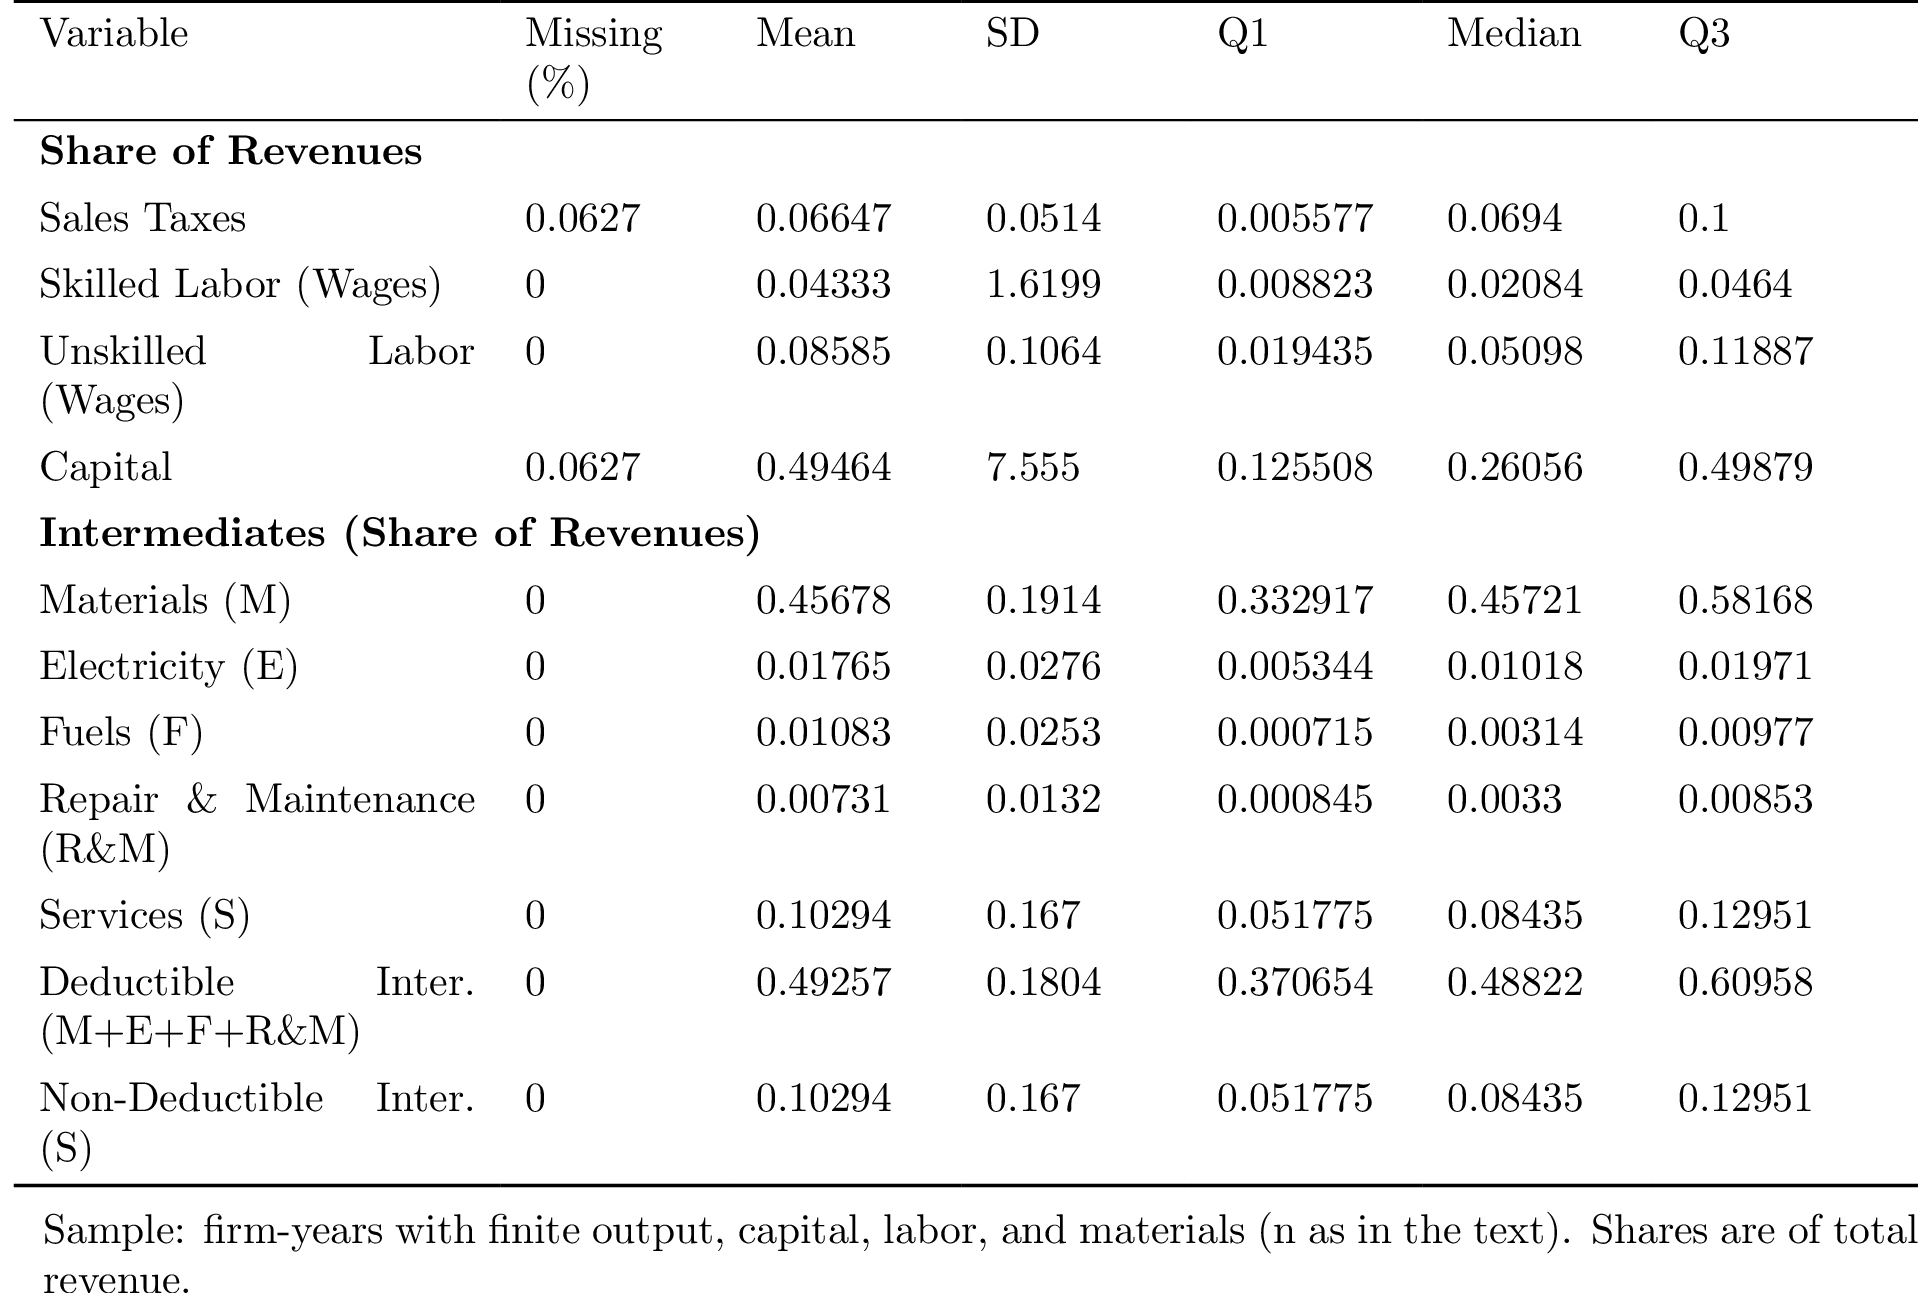
\includegraphics[keepaspectratio]{tables/ch03-summary-stats.png}}

}

\end{table}%

\begin{itemize}
\tightlist
\item
  Two groups of shares (of revenue): direct cost shares (sales tax,
  skilled/unskilled labor wages, capital) and the
  materials/intermediates decomposition (materials, electricity, fuels,
  repair \& maintenance, services, deductible vs.~non-deductible
  intermediates). The materials/deductible split matters later
  (Chapter~\ref{sec-testing}): only deductible intermediates carry an
  overreporting incentive.
\item
  Note for the write-up, not a rendering issue: skilled-labor-share SD
  (1.62) is far above its own mean/Q3 --- a small number of extreme
  outliers in that one column. Decide whether to mention/trim; not
  addressed in the table itself.
\end{itemize}

\section{Juridical organization}\label{sec-setting-jo}

\begin{table}

\caption{\label{tbl-jo-summary}Juridical organization, manufacturing
firms in Colombia (1981--1991).}

\centering{

\pandocbounded{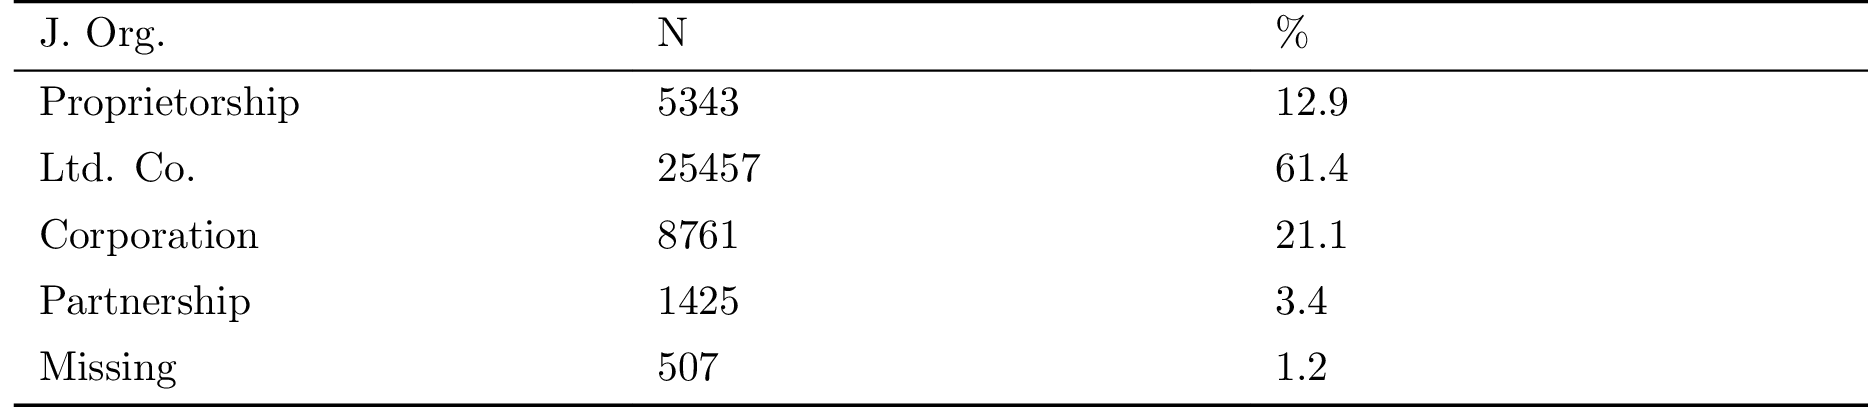
\includegraphics[keepaspectratio]{tables/ch03-jo-summary.png}}

}

\end{table}%

\begin{itemize}
\tightlist
\item
  Five types in the data; four kept in the analysis (Corporation,
  Limited Liability Company, Partnership, Proprietorship). Others
  (cooperatives, community/state enterprises) excluded --- not
  profit-driven, no evasion incentive of the kind modeled.
\item
  Definitions (safe to copy from \texttt{80-colombia.qmd}, institutional
  facts, not model output):

  \begin{itemize}
  \tightlist
  \item
    \textbf{Corporation} (\emph{sociedad anónima}): capital association,
    \(N\ge5\) shareholders, tradable shares, liability limited to
    capital, supervised by the Superintendent of Corporations with a
    mandatory auditor.
  \item
    \textbf{Limited liability company} (\emph{sociedad de
    responsabilidad limitada}): \(2\le N\le20\) (25 in the 1992 EAM
    documentation), non-tradable shares, liability limited to capital.
  \item
    \textbf{Partnership} (\emph{sociedad colectiva} and variants):
    \(N\ge2\), full/joint liability, not a capital association.
  \item
    \textbf{Proprietorship}: single individual, full liability.
  \end{itemize}
\item
  Corporate Income Tax (CIT) by type: Corporations 40\% on distributed
  dividends; Partnerships and LLCs 20\% on profits (whether distributed
  or not); Proprietorships on the graduated individual schedule (56
  brackets, 0.5\%-51\%).
\item
  Since 1974, a minimum presumptive income (8\% of net wealth) applied
  to individuals and juridical organizations except LLCs. Some
  industries/regions had CIT exempted or reduced (airlines, publishing,
  reforestation; ``frontier'' regions).
\end{itemize}

\begin{tcolorbox}[enhanced jigsaw, arc=.35mm, bottomrule=.15mm, bottomtitle=1mm, breakable, colback=white, colbacktitle=quarto-callout-note-color!10!white, colframe=quarto-callout-note-color-frame, coltitle=black, left=2mm, leftrule=.75mm, opacityback=0, opacitybacktitle=0.6, rightrule=.15mm, title=\textcolor{quarto-callout-note-color}{\faInfo}\hspace{0.5em}{Note}, titlerule=0mm, toprule=.15mm, toptitle=1mm]

Institutional summary table (rates/liability/capital/owners by type) ---
kept as a plain markdown table, not a generated PNG, since it states
fixed institutional facts rather than computed statistics:

{\def\LTcaptype{none} % do not increment counter
\begin{longtable}[]{@{}
  >{\centering\arraybackslash}p{(\linewidth - 8\tabcolsep) * \real{0.1818}}
  >{\centering\arraybackslash}p{(\linewidth - 8\tabcolsep) * \real{0.2727}}
  >{\centering\arraybackslash}p{(\linewidth - 8\tabcolsep) * \real{0.1818}}
  >{\centering\arraybackslash}p{(\linewidth - 8\tabcolsep) * \real{0.1818}}
  >{\centering\arraybackslash}p{(\linewidth - 8\tabcolsep) * \real{0.1818}}@{}}
\toprule\noalign{}
\begin{minipage}[b]{\linewidth}\centering
Organization
\end{minipage} & \begin{minipage}[b]{\linewidth}\centering
Corporate Income Tax
\end{minipage} & \begin{minipage}[b]{\linewidth}\centering
Liability
\end{minipage} & \begin{minipage}[b]{\linewidth}\centering
Capital
\end{minipage} & \begin{minipage}[b]{\linewidth}\centering
Owners
\end{minipage} \\
\midrule\noalign{}
\endhead
\bottomrule\noalign{}
\endlastfoot
Corporation & 40\% (on distributed dividends) & Limited to capital
participation & Tradable capital shares & \(N\ge5\) \\
Limited Co. & 20\% (on profits) & Limited to capital participation &
Non-tradable capital shares & \(2\le N \le 20\ (25)\) \\
Partnership & 20\% (on profits) & Full & Not a capital association &
\(N\ge2\) \\
Proprietorship & Individual Income Tax & Full & Owner & \(N=1\) \\
\end{longtable}
}

\end{tcolorbox}

\section{Sales tax}\label{sec-setting-st}

\begin{itemize}
\tightlist
\item
  Targeted manufacturing (finished goods, imports). Since 1974, credit
  for tax paid on purchases (except capital goods) --- a VAT in
  substance.
\item
  Basic rate 15\%; preferential 6\% for clothing, footwear,
  popular-housing inputs; 35\% on luxury goods. Exports, foodstuffs,
  drugs, textbooks excluded from the start, along with
  capital/agricultural inputs and transport/agricultural equipment.
\item
  This is the rate the 1983 reform changed (Chapter~\ref{sec-fiscal}):
  most ST-liable industries moved from 6\% to 10\%; ST-exempt industries
  stayed exempt. State this here as background; the reform and its
  effect on evasion belong to Chapter~\ref{sec-fiscal}, not here.
\end{itemize}

\section{Why corporations are the least likely
evaders}\label{sec-setting-corp-evasion}

\begin{itemize}
\tightlist
\item
  Three institutional reasons (from \texttt{80-colombia.qmd}'s
  discussion), each mapped to a modeling choice:

  \begin{enumerate}
  \def\labelenumi{\arabic{enumi}.}
  \tightlist
  \item
    Mandatory auditor and Superintendent oversight \(\to\) higher
    detection probability \(q\) for corps in the model.
  \item
    Tradable shares create a market-value cost to underreporting profits
    \(\to\) an implicit cost channel outside \(\kappa(e,\omega)\), not
    separately modeled.
  \item
    CIT on distributed (not accrued) dividends gives corporations a
    timing margin ordinary profit-shifting doesn't have.
  \end{enumerate}
\item
  This is the institutional justification for treating corps as \(e=0\)
  in stage 1 (Chapter~\ref{sec-testing},
  Chapter~\ref{sec-deconvolution}) --- state it here once, reference it
  there.
\item
  Proprietorships, partnerships and LLCs face both CIT and ST incentives
  to overreport; incentives vary by industry (ST rate) and by juridical
  organization within industry (CIT rate) --- sets up
  Chapter~\ref{sec-fiscal}'s identification strategy.
\end{itemize}

\section{Top industries}\label{sec-setting-industries}

\begin{table}

\caption{\label{tbl-top-inds-rev}Top 10 industries in Colombia by
revenue.}

\centering{

\pandocbounded{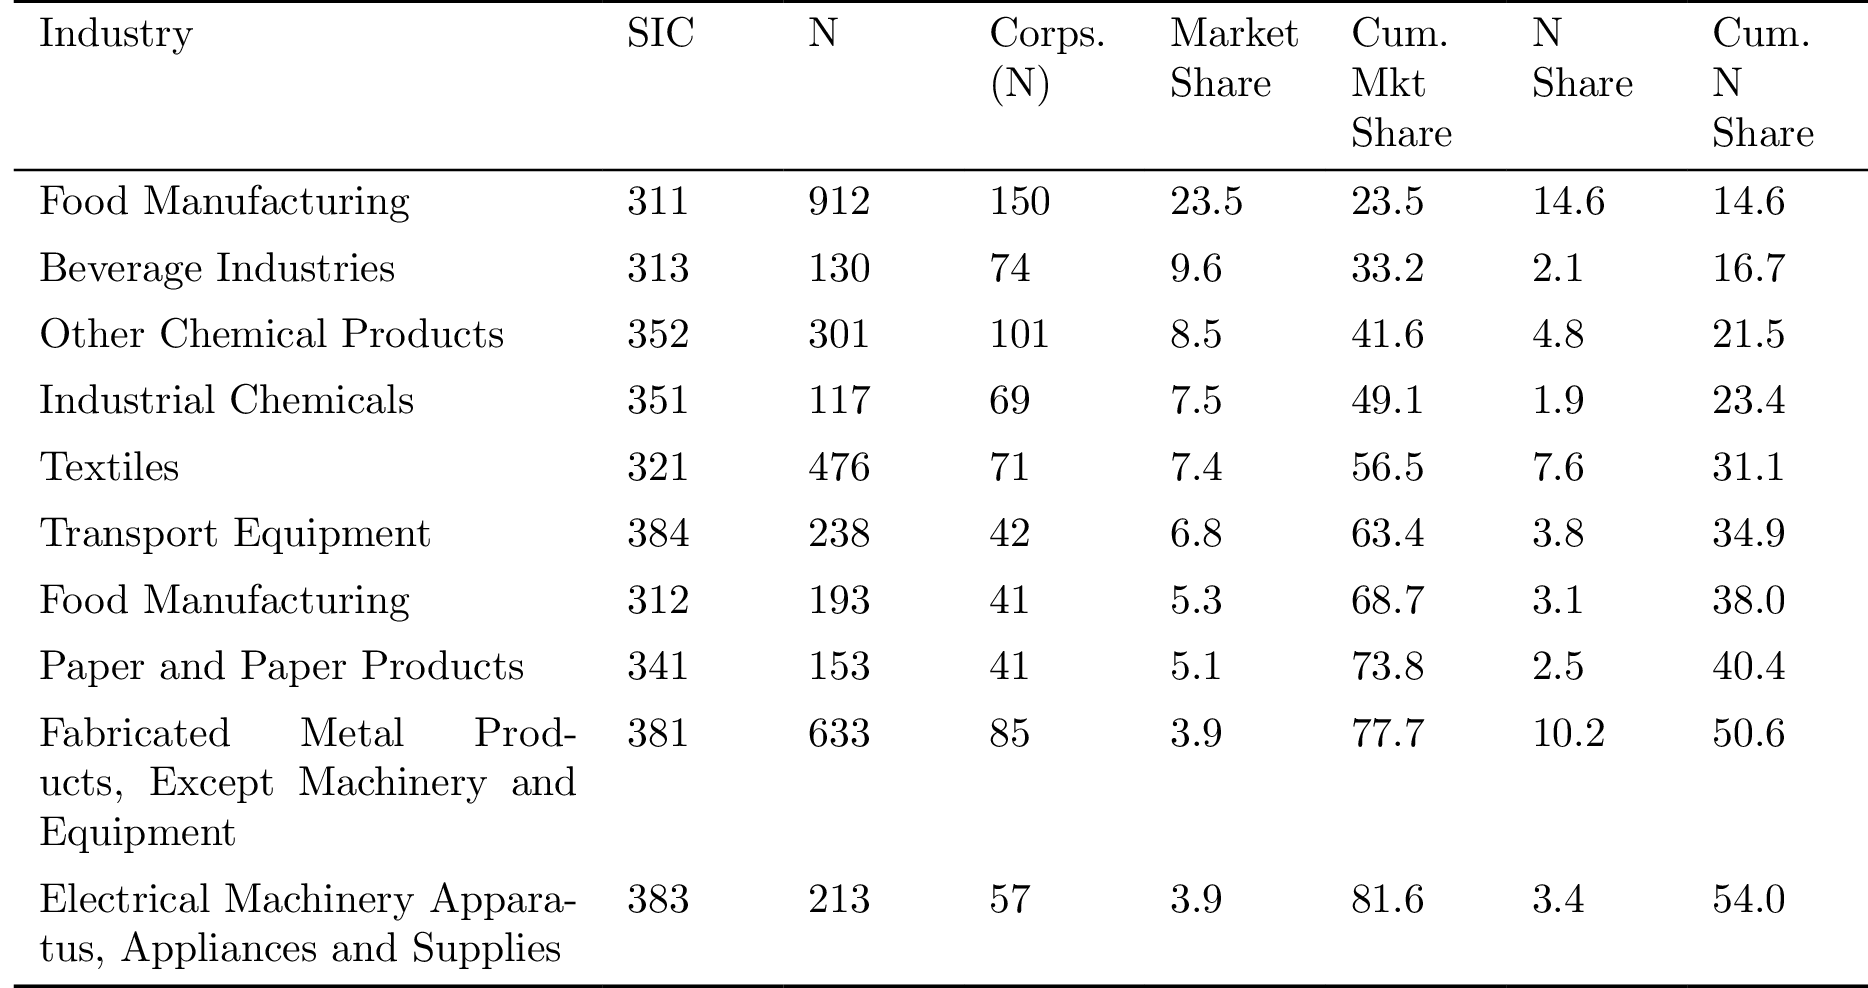
\includegraphics[keepaspectratio]{tables/ch03-top-industries.png}}

}

\end{table}%

\begin{table}

\caption{\label{tbl-corps-by-inds}Corporations by industry. Top 20
industries in Colombia by number of firms.}

\centering{

\pandocbounded{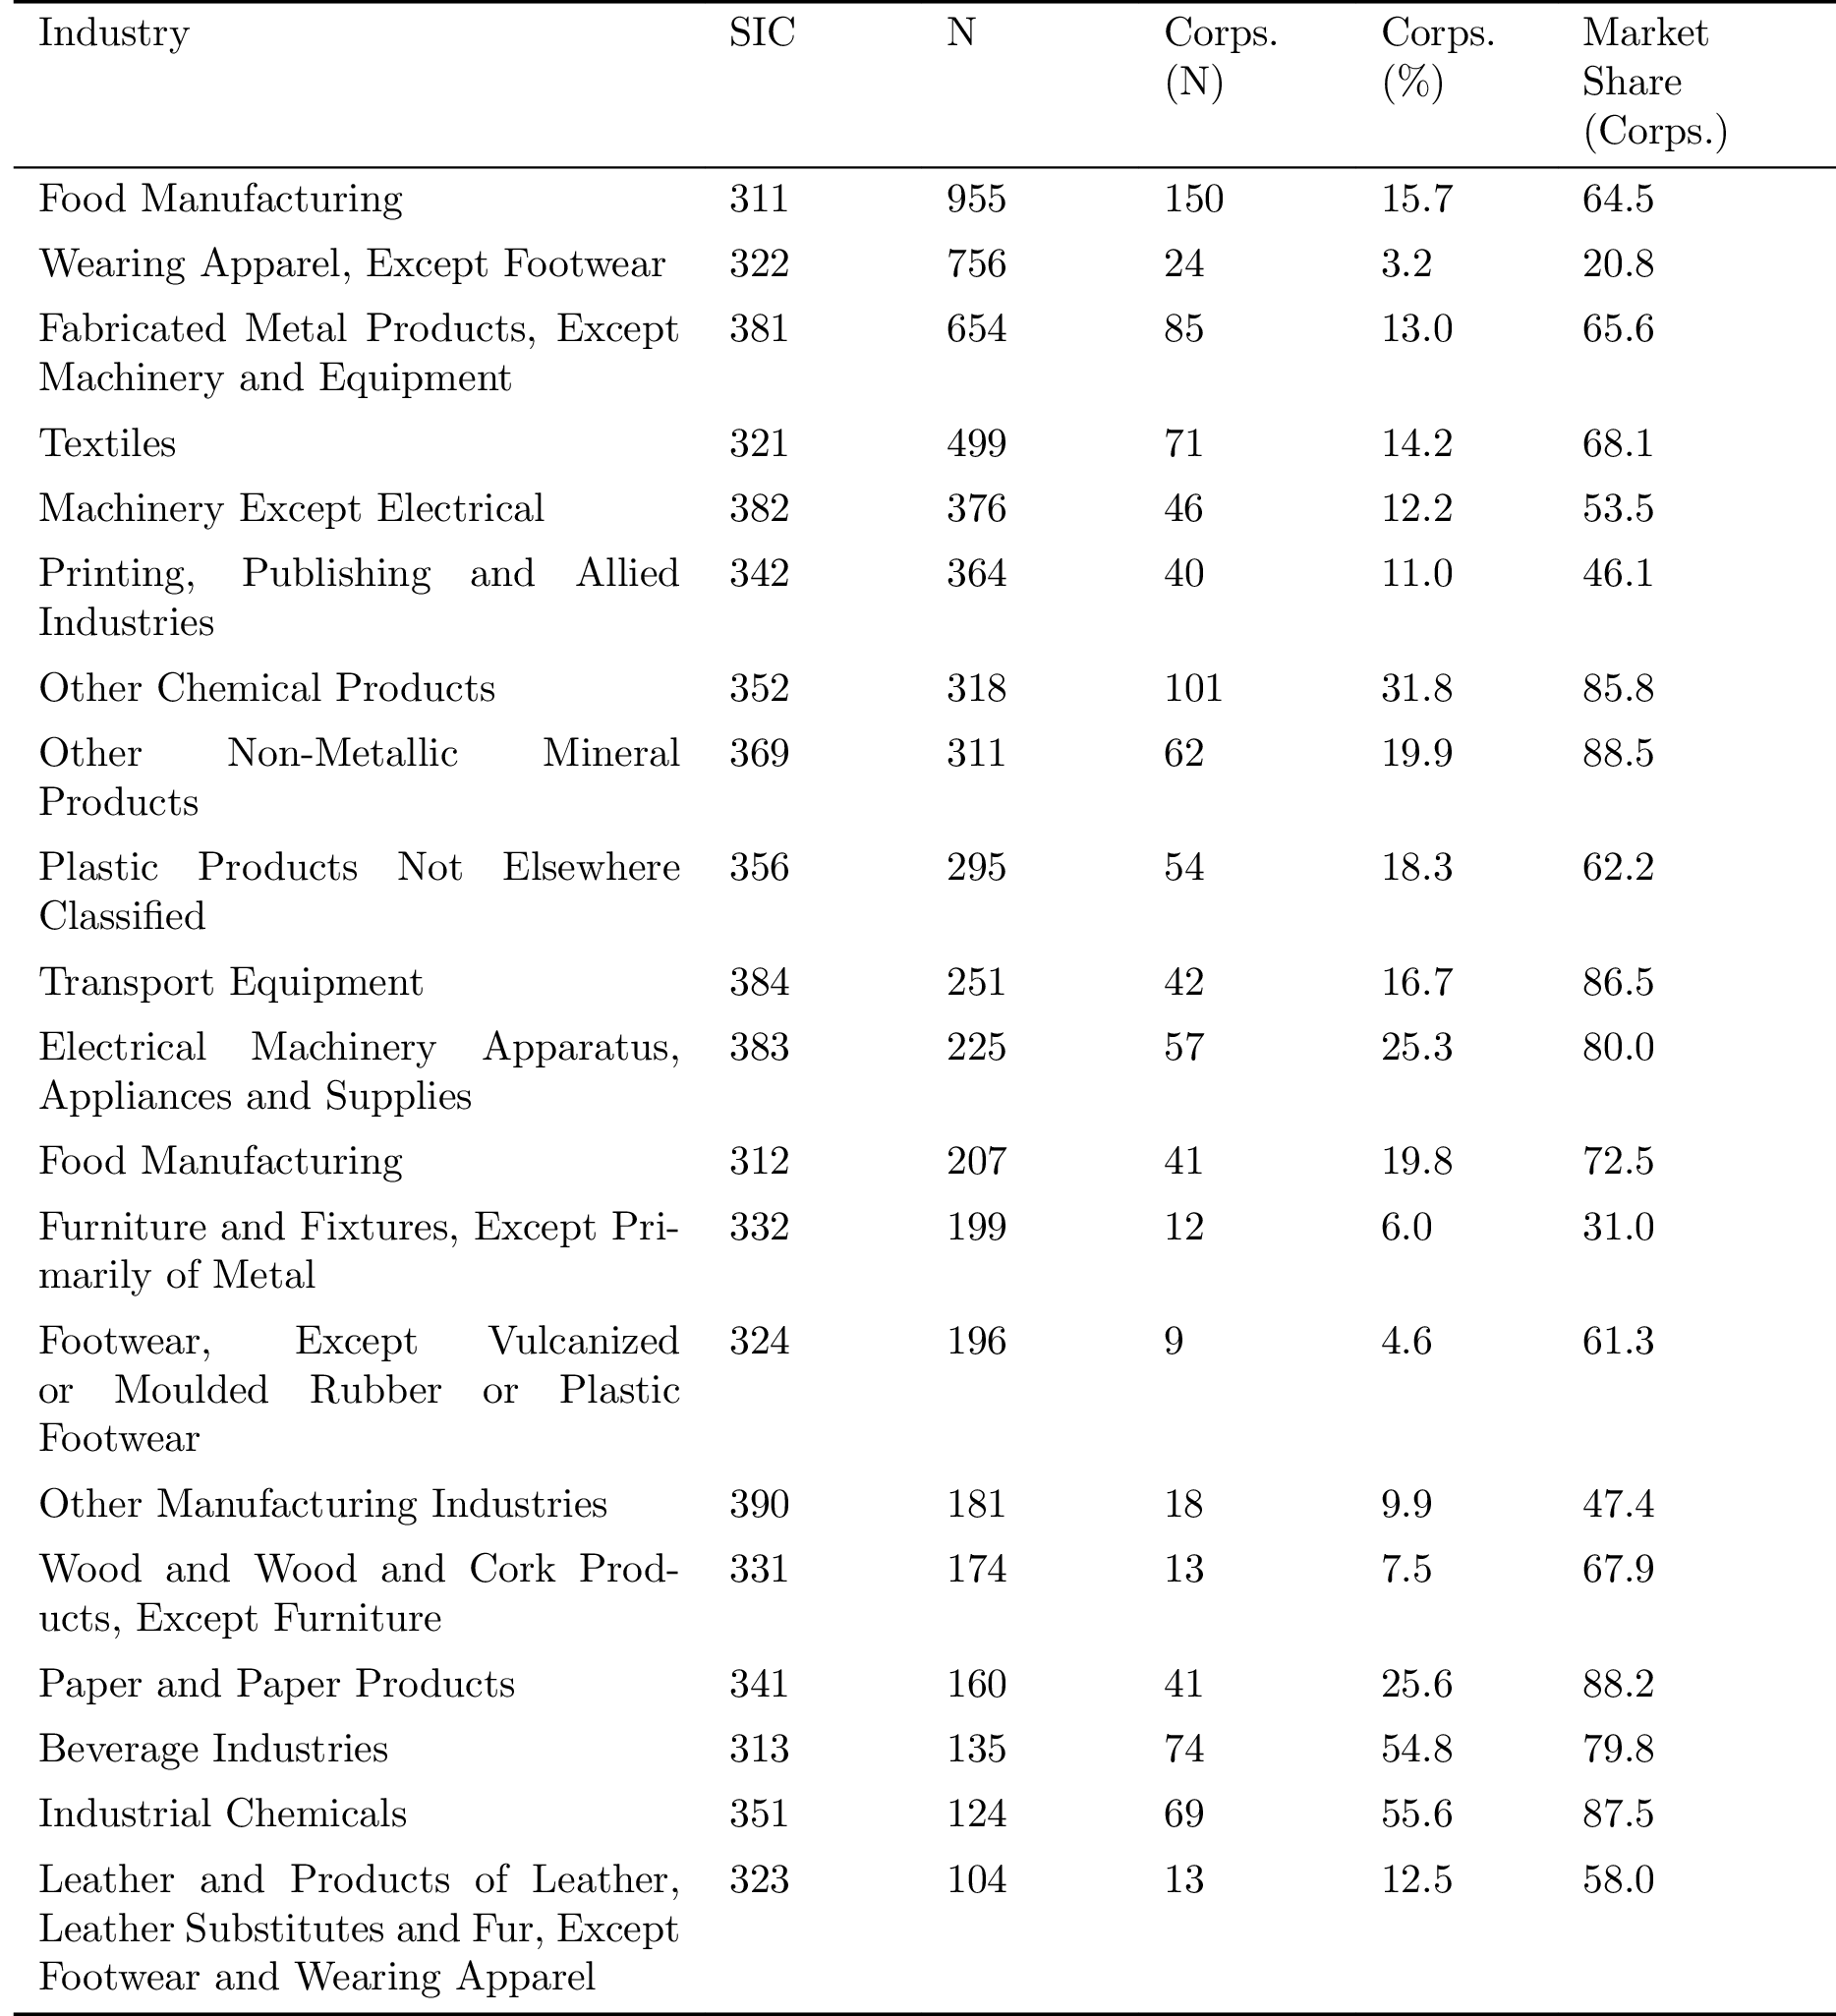
\includegraphics[keepaspectratio]{tables/ch03-corps-by-industry.png}}

}

\end{table}%

\begin{itemize}
\tightlist
\item
  UPDATE: one or two sentences on what these show (revenue
  concentration; corporate share varies a lot by industry) --- sets up
  why industry fixed effects matter in Chapter~\ref{sec-fiscal} and why
  some industries carry more weight in Chapter~\ref{sec-pf},
  Chapter~\ref{sec-counterfactual}.
\end{itemize}

\section{Open items}\label{open-items}

\begin{itemize}
\tightlist
\item[$\square$]
  Fill sample-size/coverage sentence in Section~\ref{sec-setting-data}
  with the actual filtered N (currently only in the table).
\item[$\square$]
  Decide whether to note/trim the skilled-labor-share outliers flagged
  under Table~\ref{tbl-sum-stats}.
\item[$\square$]
  One or two sentences for Table~\ref{tbl-top-inds-rev} /
  Table~\ref{tbl-corps-by-inds} (marked UPDATE above).
\item[$\square$]
  Confirm the institutional JO/CIT/ST facts here still match how they're
  used in \texttt{80-colombia.qmd}; this chapter is a close copy of that
  file's content, reorganized around what later chapters need.
\end{itemize}

\bookmarksetup{startatroot}

\chapter{Testing for Tax Evasion through
Overreporting}\label{sec-testing}

\bookmarksetup{startatroot}

\chapter{Deconvolving Tax Evasion}\label{sec-deconvolution}

\bookmarksetup{startatroot}

\chapter{Production Function Parameters and Productivity}\label{sec-pf}

\section{Production function
estimates}\label{production-function-estimates}

\begin{table}

\caption{\label{tbl-pf-comparison}Production function parameters: joint
efficient GMM (\(m^*_{it-1}+\tilde{\mathcal W}_{it-2}\), \(\beta\)
fixed) vs.~uncorrected GNR and OLS. \(\hat\alpha_K,\hat\alpha_L\) report
both 95\% test-inversion regions (sharp/conservative).}

\centering{

\pandocbounded{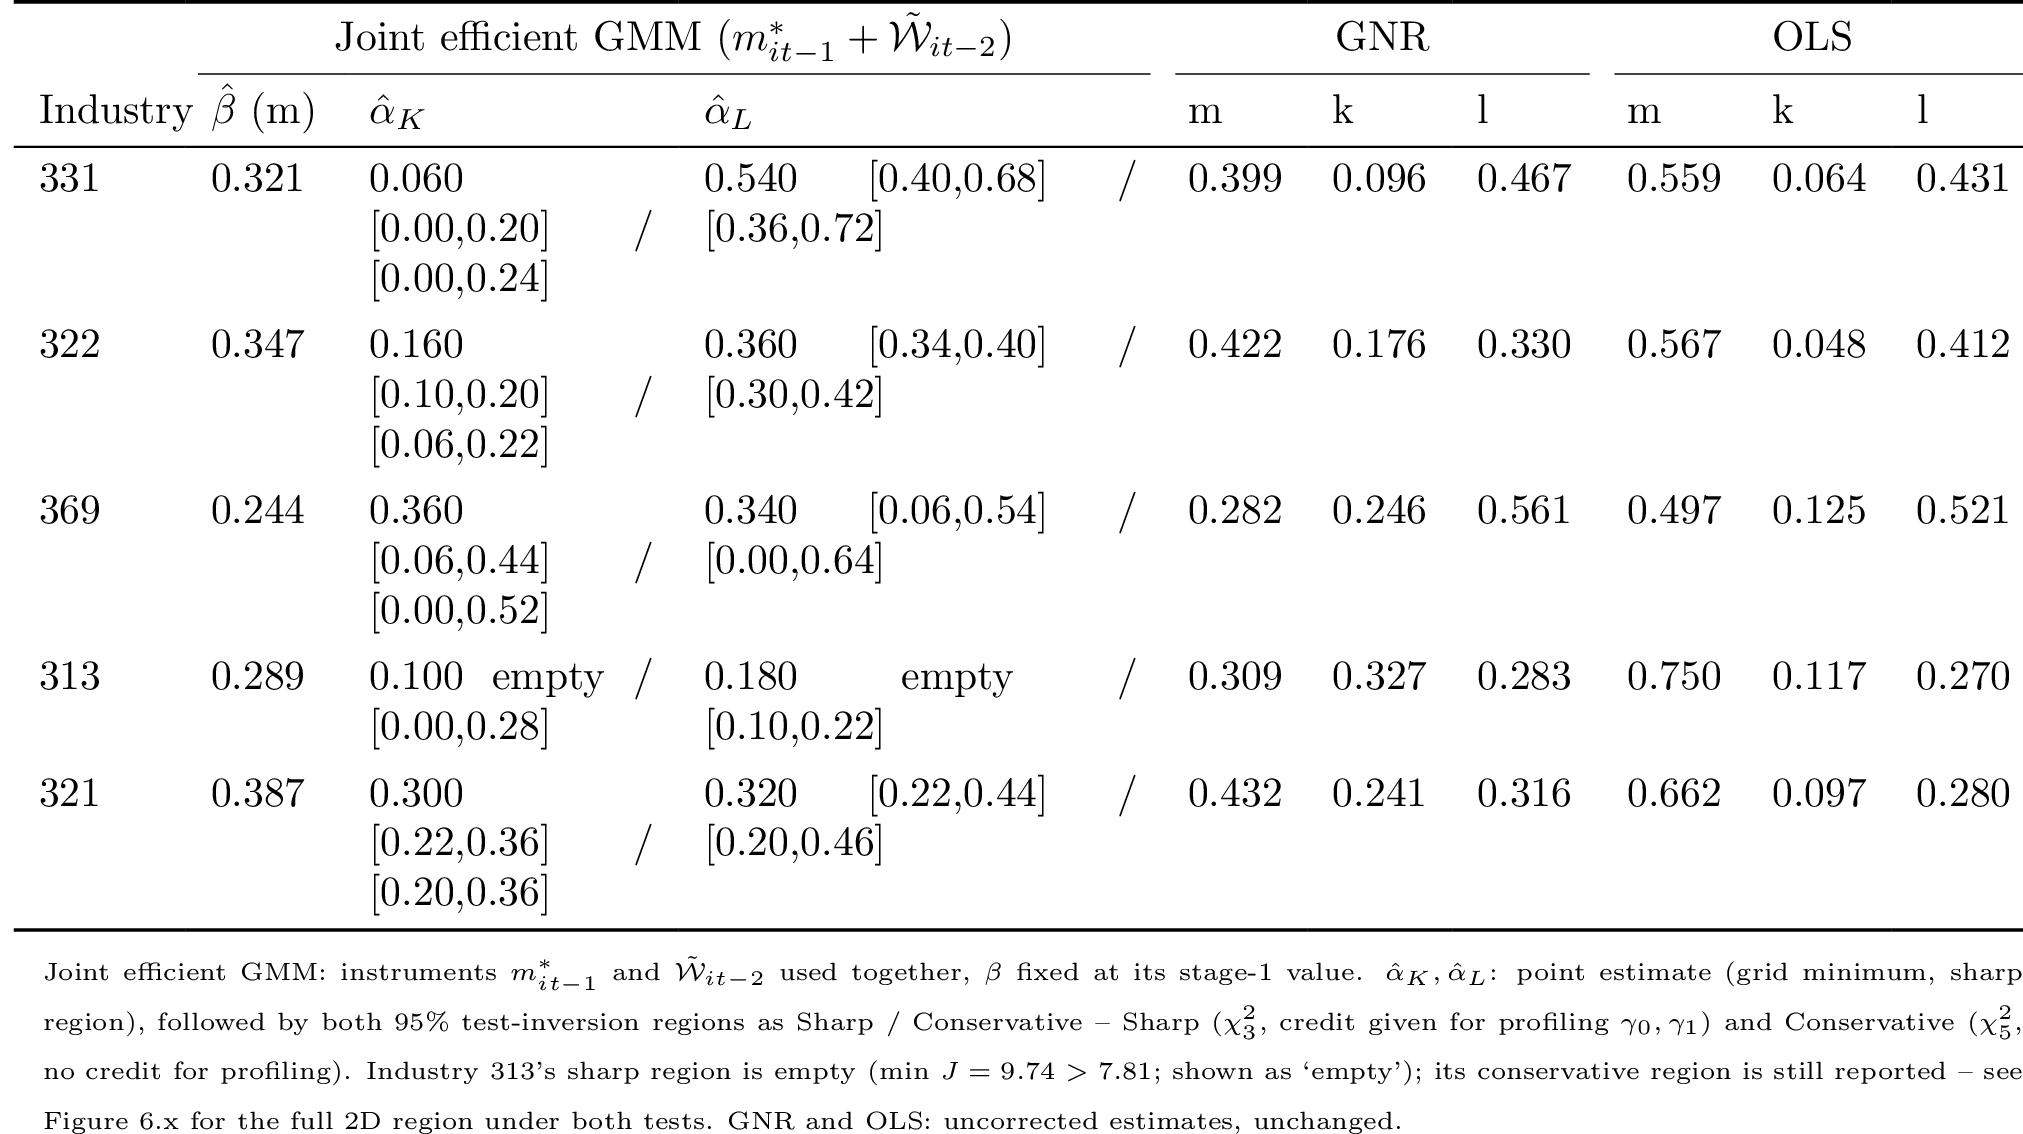
\includegraphics[keepaspectratio]{tables/ch06-pf-comparison.png}}

}

\end{table}%

\begin{figure}

\centering{

\pandocbounded{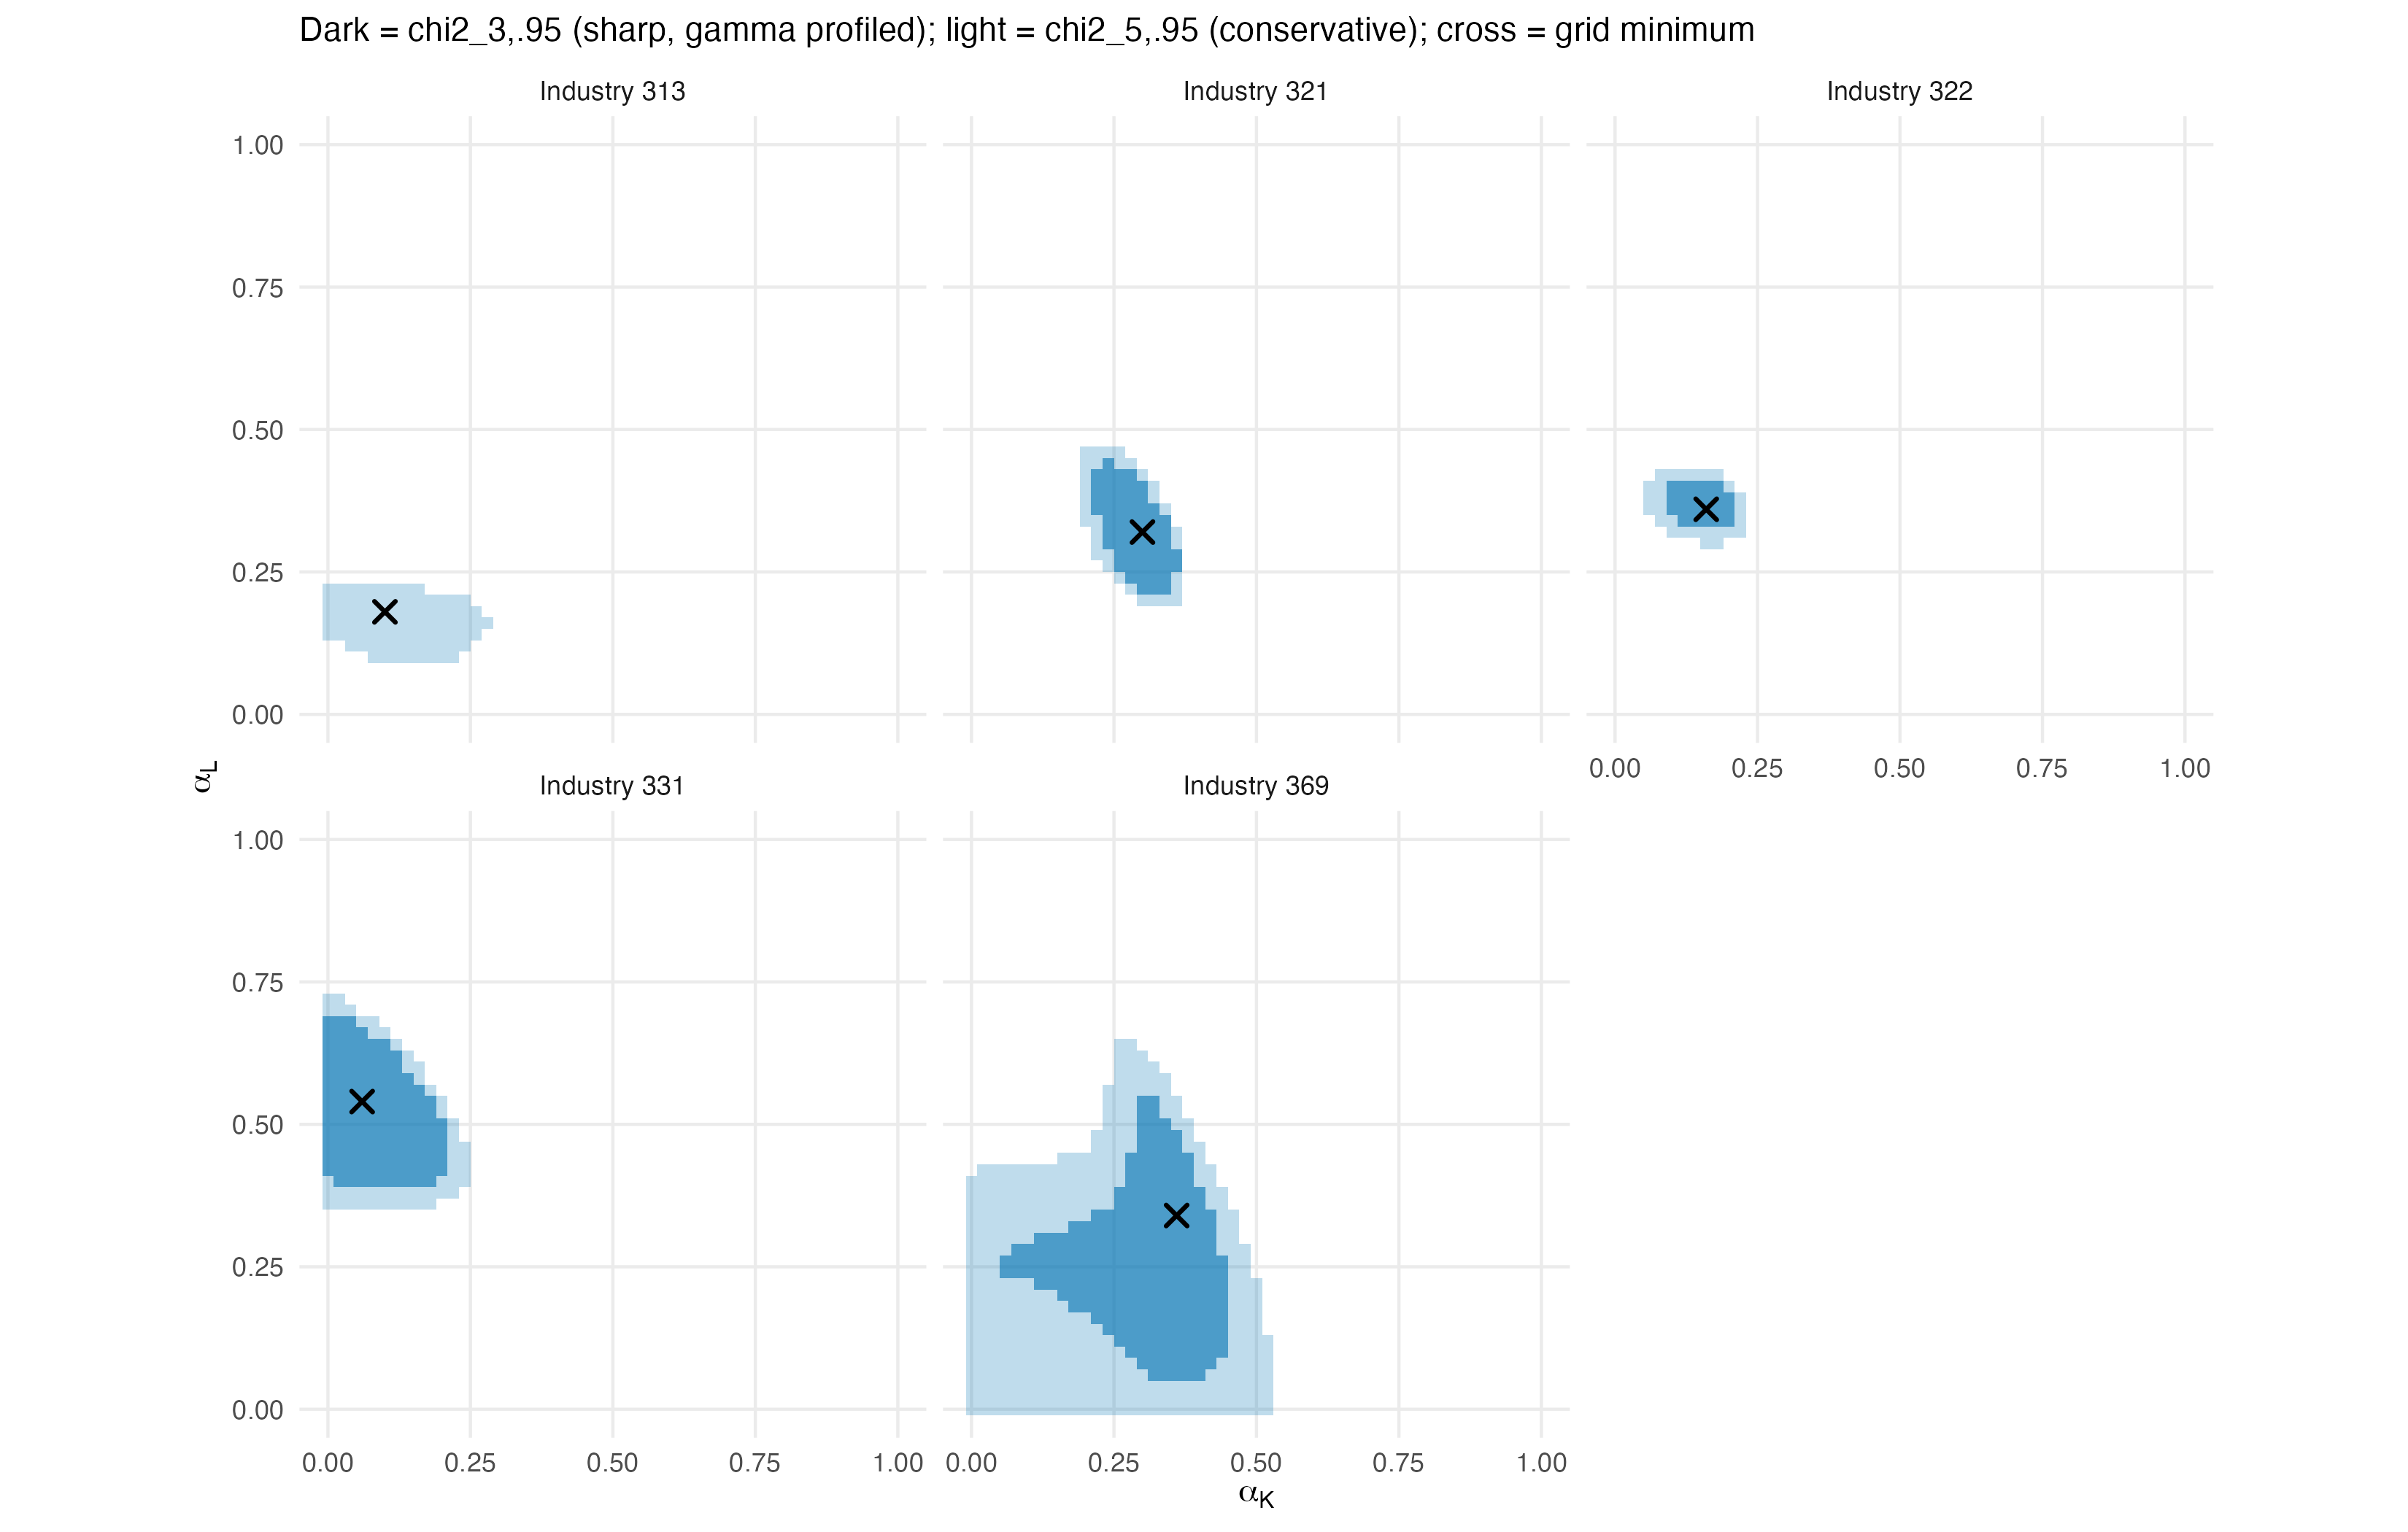
\includegraphics[keepaspectratio]{figures/ch06-pf-testinv-regions.png}}

}

\caption{\label{fig-pf-testinv-regions}Test-inversion regions for
\((\alpha_K,\alpha_L)\), sharp and conservative tests.}

\end{figure}%

\section{Robustness: single-tax vs.~net-of-tax first
stage}\label{robustness-single-tax-vs.-net-of-tax-first-stage}

\begin{table}

\caption{\label{tbl-beta-net-tax}\(\hat\beta\) under the gross
(approved, headline) vs.~net-of-tax first stage, 5 headline industries.}

\centering{

\pandocbounded{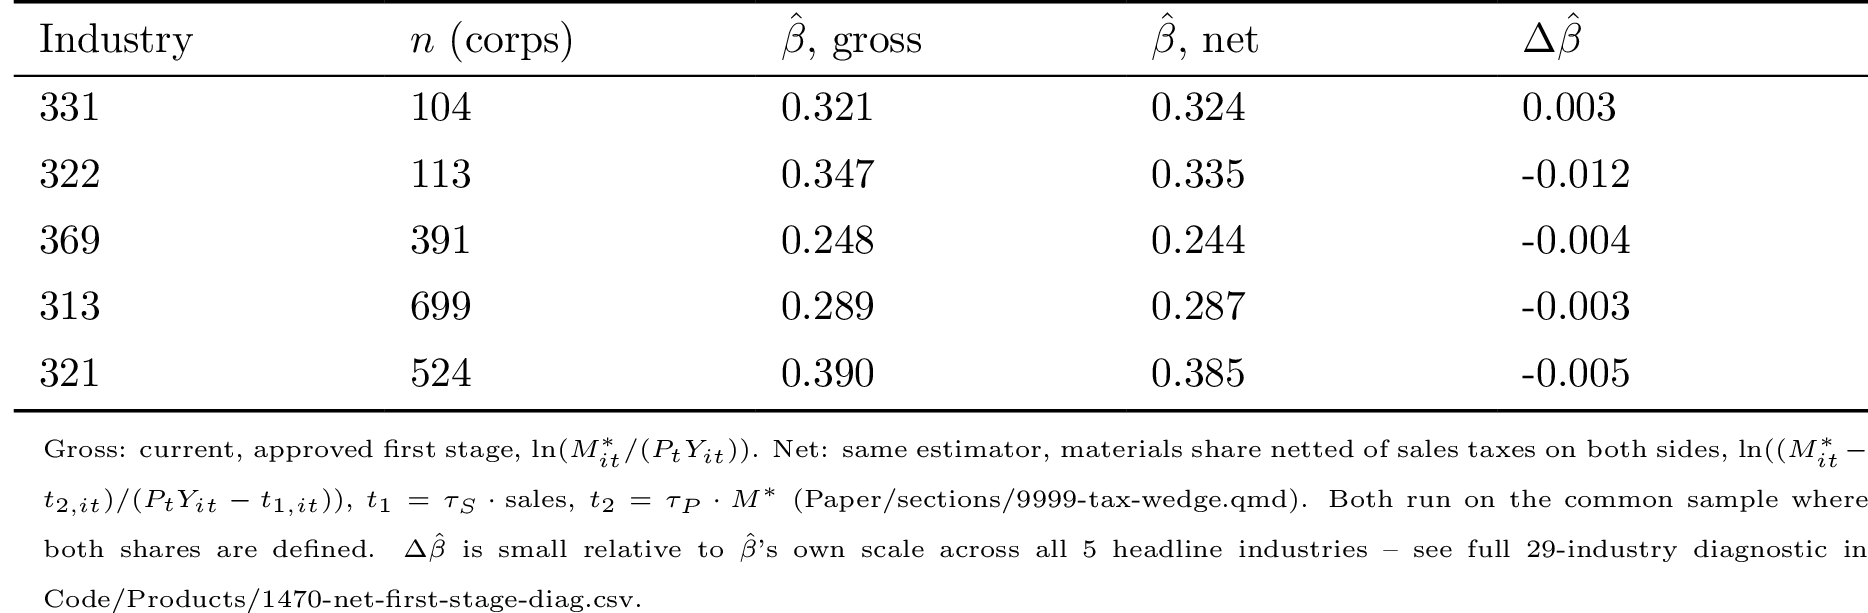
\includegraphics[keepaspectratio]{tables/ch06-beta-net-tax.png}}

}

\end{table}%

\bookmarksetup{startatroot}

\chapter{Fiscal Policy Evaluation: The 1983 Reform}\label{sec-fiscal}

\section{Role of this chapter}\label{role-of-this-chapter-1}

\begin{itemize}
\tightlist
\item
  Reduced-form evidence that overreporting responds to a change in tax
  incentives; this is the empirical anchor for the model's key
  comparative static, \(\partial e^*/\partial\tau_P>0\)
  (Chapter~\ref{sec-model}).
\item
  The sign cannot be checked by regressing \(\mathcal V_{it}\) on
  \(\tau_{P,it}\) (both are built from the same \(M^*_{it}\), so the
  link is mechanical). The 1983 reform is the clean way to test it.
\item
  Feeds the identification argument for \(\lambda\) in
  Chapter~\ref{sec-counterfactual}: variation in \(\tau_P\rho_t\) is
  what moves evasion.
\item
  UPDATE: decide framing for the thesis: motivation for the structural
  model (``reduced form showed X, the model's Y rationalizes X'').
\end{itemize}

\section{The reform and the incentives}\label{sec-reform}

\begin{itemize}
\tightlist
\item
  1983 reform raised the Sales Tax (ST) rate from 6\% to 10\% for most
  industries; ST-exempt industries stayed exempt.
\item
  Across juridical organizations (JO) within industries, Corporate
  Income Tax (CIT) moved differently:

  \begin{itemize}
  \tightlist
  \item
    Proprietorships (PRT): CIT up about 8\% on average (via individual
    income tax).
  \item
    Limited liability companies (LLC): CIT down 2 points, 20\% to 18\%.
  \end{itemize}
\item
  Both taxes create incentives to overreport inputs (a higher reported
  cost lowers the base). ST-liable industries face ST and CIT
  incentives; ST-exempt industries face CIT only.
\item
  Expected sign: ST-liable firms should increase overreporting (ST up).
  CIT effect ambiguous (PRT up, LLC slightly down).
\item
  UPDATE: Paper (\texttt{965-DiD}) also covers the 1986 reform; the
  slides only mention it in a commented line. Decide whether 1986 stays.
\item
  Institutional details (6\% to 10\%, CIT rates) come from
  Chapter~\ref{sec-setting}; do not repeat them at length here.
\end{itemize}

\section{Empirical approach}\label{sec-fiscal-approach}

\begin{itemize}
\tightlist
\item
  Corporations are truth-reporters:
  \(s^C_{ijt}=\gamma_j-\varepsilon_{ijt}\) (\(s\) = materials share of
  sales, \(\gamma_j\) = industry output elasticity of materials in the
  Cobb-Douglas case).
\item
  Unincorporated firms evade:
  \(s^N_{ijt}=\gamma_j+e_{ijt}-\varepsilon_{ijt}\) (here \(e\) is the
  overreporting share in the same units as \(s\); footnote the notation
  link to the model's \(u\)).
\item
  Stacking with \(D^N_{ijt}\):
  \(s_{ijt}=\gamma_j+D^N_{ijt}e_{ijt}-\varepsilon_{ijt}\).
\item
  Identifies the average overreporting
  \(\mu=E[s\mid D^N=1]-E[s\mid D^N=0]\).
\item
  Levels regression:
  \(s_{ijt}=\gamma_j+\sum_{t=1981}^{1991}\mu_tD^N_{ijt}+\eta_{ijt}\),
  \(\gamma_j\) = industry fixed effects.
\item
  Differences relative to 1983:
  \(s_{ijt}=\mu D^N_{ijt}+\sum_{t\ne1983}\Delta_tD^N_{ijt}+\gamma_j+\eta_{ijt}\),
  where \(\Delta_t=\mu_t-\mu_{1983}\).
\item
  Splitting by industry liability, with \(D^E\) (exempt) and \(D^L\)
  (liable), \(D^E+D^L=1\):

  \begin{itemize}
  \tightlist
  \item
    Exempt: \(\mu^{CIT}_E\); liable: \(\mu^{ST+CIT}_L\).
  \item
    If \(\mu^{CIT}_E=\mu^{CIT}_L\), the ST-only response \(\mu^{ST}_L\)
    is identified. State this as an assumption and discuss plausibility.
  \end{itemize}
\item
  Splitting further by JO (LLC vs proprietorship) gives four groups,
  each with its own \(\Delta_t\) path.
\end{itemize}

\section{Results: all unincorporated firms}\label{sec-fiscal-all}

\begin{figure}

\centering{

\pandocbounded{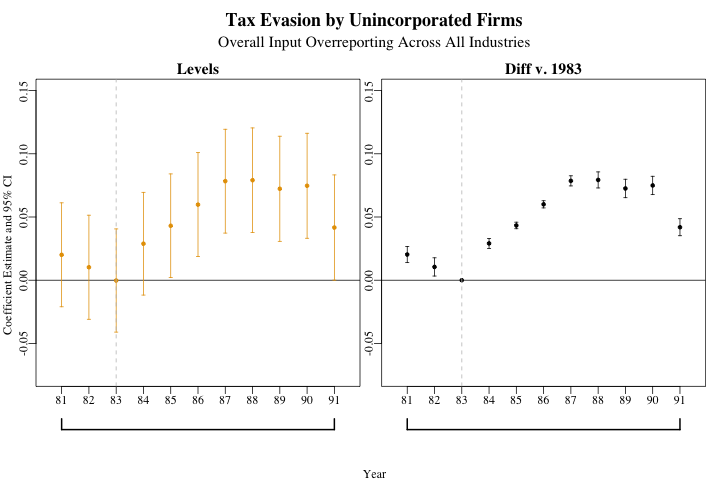
\includegraphics[keepaspectratio]{figures/ch07-fiscal-all-unincorp.png}}

}

\caption{\label{fig-fiscal-all}Overreporting of unincorporated firms
relative to 1983.}

\end{figure}%

\begin{itemize}
\tightlist
\item
  Overreporting rises gradually after the reform and reaches an average
  of about 8\% in 1987, stable until 1990.
\item
  Levels have wide standard errors (heterogeneity across firms in tax
  rate, perceived detection probability and evasion cost); differences
  relative to 1983 are tight, so the heterogeneity looks constant over
  time.
\item
  FILL: point estimates and standard errors for 1984-1991 from
  \texttt{921-DD2.R} output.
\end{itemize}

\section{Results: ST-liable vs.~ST-exempt
industries}\label{sec-fiscal-liable}

\begin{figure}

\centering{

\pandocbounded{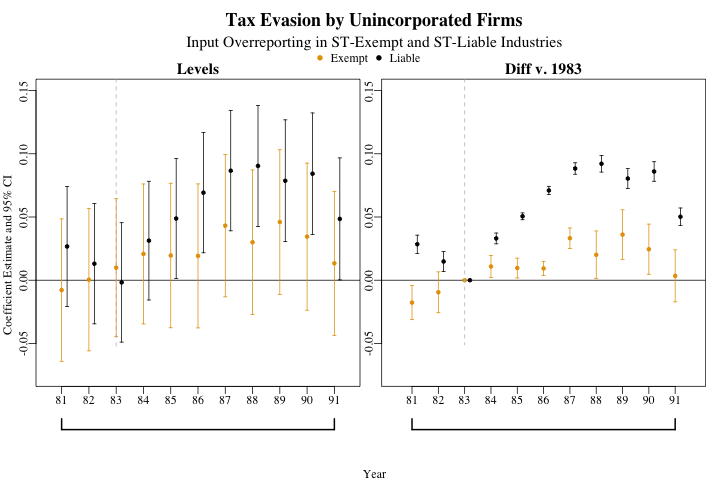
\includegraphics[keepaspectratio]{figures/ch07-fiscal-liable-vs-exempt.png}}

}

\caption{\label{fig-fiscal-liable}Firms facing larger incentives evade
more.}

\end{figure}%

\begin{itemize}
\tightlist
\item
  ST-liable: overreporting rises gradually until 1987, then stabilizes
  through 1990.
\item
  ST-exempt: smaller but significant increase after 1983, and another
  increase between 1987 and 1990.
\item
  The increase is larger for ST-liable firms, the group most affected by
  the reform.
\end{itemize}

\section{Results: LLCs vs.~proprietorships}\label{sec-fiscal-jo}

\begin{figure}

\centering{

\pandocbounded{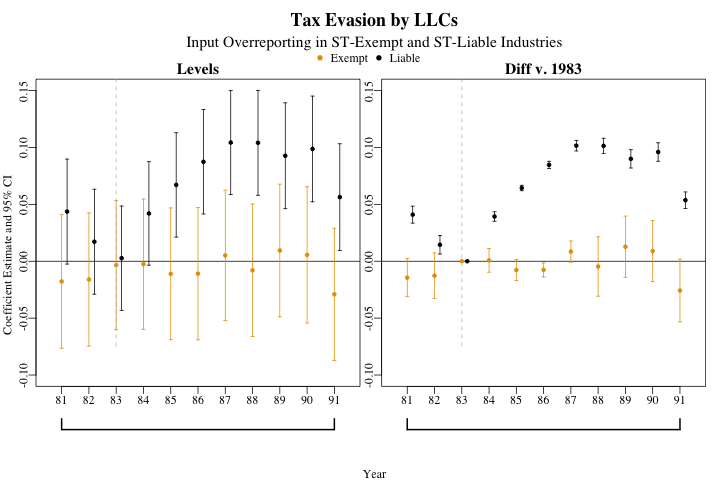
\includegraphics[keepaspectratio]{figures/ch07-fiscal-llc.png}}

}

\caption{\label{fig-fiscal-llc}LLCs.}

\end{figure}%

\begin{figure}

\centering{

\pandocbounded{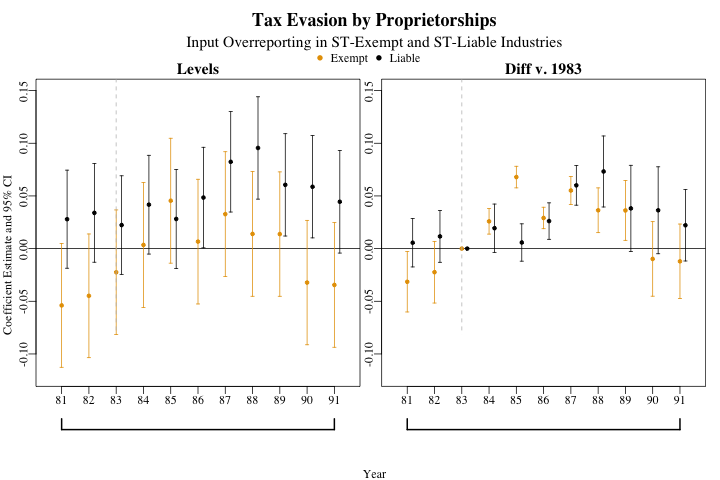
\includegraphics[keepaspectratio]{figures/ch07-fiscal-prt.png}}

}

\caption{\label{fig-fiscal-prt}Proprietorships.}

\end{figure}%

\begin{itemize}
\tightlist
\item
  LLCs in ST-liable industries: significant increase (consistent with
  the ST increase).
\item
  LLCs in ST-exempt industries: no significant change, so the small CIT
  cut did not reduce overreporting.
\item
  Proprietorships in ST-exempt industries: moderate significant increase
  (consistent with the CIT increase).
\item
  Proprietorships in ST-liable industries: no change in 1984-1985, an
  increase in 1986-1989. Larger standard errors, more heterogeneous
  response (workshops vs.~young entrepreneurs).
\item
  UPDATE: the 1986-1989 rise may reflect the 1986 reform; keep or drop
  depending on the 1986 decision above.
\end{itemize}

\section{Takeaways and link to the structural
model}\label{sec-fiscal-takeaways}

\begin{itemize}
\tightlist
\item
  Firms overreport inputs more after increases in ST and CIT; larger
  increases give larger responses.
\item
  No significant decrease when incentives fall (LLCs in ST-exempt
  industries): suggests an asymmetric response. Connects to the
  counterfactual asymmetry (increases detectable at +0.5\%, cuts only at
  -8\%, Section~\ref{sec-cf-results}), but that asymmetry is a model
  implication, not this chapter's reduced-form finding; say so
  explicitly.
\item
  Bridge to Chapter~\ref{sec-counterfactual}: the model needs
  \(\tau_P\rho_t\) variation to identify \(\lambda\); this chapter shows
  that variation moves overreporting in the predicted direction.
\end{itemize}

\section{Open items}\label{open-items-1}

\begin{itemize}
\tightlist
\item[$\square$]
  Choose which Paper DiD sections survive (\texttt{965-DiD},
  \texttt{966-DiD-txrt}, \texttt{98-fiscal-ref-col},
  \texttt{961-over-time}); slides only cover the 921-2 specification.
\item[$\square$]
  Decide whether the 1986 reform and the 1990 reform stay.
\item[$\square$]
  Move the 921-2 figures to \texttt{Code/Thesis/ch07-*.R} scripts
  (currently copied PNGs).
\item[$\square$]
  Rewrite the abstract and intro claims about this chapter
  (\texttt{Paper/Tax-Prod.qmd} abstract still says ``raised their
  overreported share significantly'').
\end{itemize}

\bookmarksetup{startatroot}

\chapter{The Counterfactual: Revenue and the Purchases-Side
Tax}\label{sec-counterfactual}

\section{Partial Equilibrium Laffer Curve}\label{sec-cf-question}

How does tax revenues change as the government changes the sales tax
rate on purchases? As the tax rate increases, the incentives to claim
additional fictitious deductions increase, but an increase in evasion
raises the probability of detection. On the flip side, a decrease in the
tax rate reduces the incentives to evade and firms start to decrease
their intensity and some firms start jumping out of evasion altogether.
Taking the current observed state, what is the marginal change in
revenue as tax changes?

I study this question using the estimates of the structural objects from
the firms' tax evasion model. With the parameters at hand, I construct a
partial equilibrium Laffer curve. The counterfactual curve allows me to
investigate how the government's tax revenue changes as sales tax rates
on purchases changes.

The results shows a downward slopping Laffer curve with a kink at the
current state. The curve shows that revenue losses would not
significantly fall from baseline unless there is a tax cut of at least
8\%. In contrast, an increase of 0.5\% will significanlty increase
revenues losses.

Given the firm's optimization problem, the government chooses the tax
rate on purchases to maximize expected tax revenue.

\begin{equation}\protect\phantomsection\label{eq-govt-rev}{
R_i(\Delta;M_i) = \tau_{S,it}P_tY_{it} - \tilde\tau_{P,it}\big[M_i+(1-q(\tilde e_i(\Delta)))\tilde e_i(\Delta)\big]
}\end{equation}

where \(\tilde\tau_{P,it}\equiv\tau_P\to(1+\Delta)\tau_P\). The first
term in Equation~\ref{eq-govt-rev} is the revenue collected from sales
taxes on sales \(\tau_{S,it}P_tY_{it}\). The second term is the credits
claimed on sales taxes on purchases, \(\tau_{P,it}\). The term includes
the firms' true inputs, \(M_{it}\), plus the counterfactual undetected
evasion,\((1-q(\tilde e_{it}(\Delta)))\tilde e_{it}(\Delta)\), at tax
rate percentage change \(\Delta\). The firm's FOC shows \(\tau_P\)
directly modifies the marginal benefit of evasion leading to changes in
the optimal evasion \(\tilde e_i(\Delta)\).

In general governments can also choose enforcement effort level, and
therefore they can affect \(q(\cdot)\). In addition, governments might
collect additional income penalizing firms caught evadin. Moreover,
firms might change their optimal true inputs because when there are two
different sales taxes on sales and purchases, the government can affect
the relative prices and thus influence output indirectly. Since we lack
information on both, we restrict our attention only to changes in tax
revenue losses due to changes in expected claims. In other words, we fix
output and optimal input decisions.

\begin{itemize}
\tightlist
\item
  Not ``what \(\Delta\) maximizes revenue?'' (an interior optimum need
  not exist) but ``what is the derivative of tax revenue with respect to
  the purchases-side credit rate at the current state?''
\item
  Holding sales-tax revenue, \(M\), \(K\), \(L\), \(\omega\),
  \(\varepsilon\) fixed; only evasion responds. A local comparative
  static, not a general-equilibrium optimal-tax result.
\item
  Two-tax-rate model: only \(\tau_P\) enters the evasion FOC; \(\tau_S\)
  never does. Shock: \(\tilde\tau_{P,it}=(1+\Delta)\tau_{P,it}\).
\item
  Revenue:
  \(R_i(\Delta;M_i)=t1_{it}-\tilde\tau_{P,it}\big[M_i+(1-q(\tilde e_i(\Delta)))\tilde e_i(\Delta)\big]\),
  with \(t1_{it}=\tau_{S,it}P_tY_{it}\) fixed; corner firms
  (\(\tau_P=0\)): \(R_i=t1_{it}-\tilde\tau_{P,it}M^*_{it}\).
\item
  Structural result (envelope theorem, any regular \(q,\kappa\)):
  \(dR/dx<0\) always with \(M\) fixed (\(x=1+\Delta\)). Revenue is a
  pure transfer between government and evaders.
\item
  Check that \(M\) does not respond (materials FOC gives \(M'(x)>0\)):
  at \(\Delta=0\), median firm, \(\hat\beta=0.387\),
  \(\hat\tau_P=0.088\), \(\hat\tau_S=0.089\),
  \(\hat\lambda=5.427\times10^{-7}\):
\end{itemize}

{\def\LTcaptype{none} % do not increment counter
\begin{longtable}[]{@{}lr@{}}
\toprule\noalign{}
term & value \\
\midrule\noalign{}
\endhead
\bottomrule\noalign{}
\endlastfoot
output-growth (new channel) & \(\approx+1.8\) \\
mechanical legit-credit & \(\approx-819\) \\
evasion response & \(\approx-80{,}655\) \\
\end{longtable}
}

Evasion dominates by about 45,000x, driven by
\(1/(2\hat\lambda)\approx921{,}000\). Holding \(M\) fixed does not
distort the answer. - Derivation goes to the appendix
(\texttt{9999-tax-wedge.qmd}).

\section{Setting}\label{setting}

\section{Estimating the model}\label{estimating-the-model}

\subsection{Setup}\label{setup-1}

Using estimates of the production function parameters from - Stage 1
(Chapter~\ref{sec-deconvolution}, Chapter~\ref{sec-pf}): corporations
(\(e=0\)) give \(\hat\beta\) and the residuals
\(\mathcal V_{it}=u_{it}-\varepsilon_{it}\),
\(\tilde{\mathcal W}_{it}=\omega_{it}+(1-\beta)\varepsilon_{it}\). -
Stage 2 estimates \(\theta=(\lambda,\delta_0,\delta_1,\delta_2)\) from
unincorporated firms. Detection \(q(e)=\min\{\lambda e,1\}\) (linear);
cost \(\kappa=e\exp\{\delta_0-\delta_1\omega+\delta_2\omega^2+\psi\}\),
U-shaped in \(\omega\) with minimum at \(\omega^*=\delta_1/2\delta_2\).
- Evasion FOC gives
\(\psi=h(e)-\delta_0+\delta_1\omega-\delta_2\omega^2\),
\(h(e)=\ln(\tau_P\rho_t)+\ln(1-2\lambda e)\); feasibility
\(e<1/(2\lambda)\). - Why not the density-based route (MSL) or naive
simulated moments: nonlinear moment in an unobservable. One paragraph
here; full argument in Appendix~\ref{sec-app-elvis} and
Appendix~\ref{sec-app-msl}.

\subsection{ELVIS estimator}\label{elvis-estimator}

\begin{itemize}
\tightlist
\item
  Schennach (2014): take true materials \(M_{it}\) as the single
  unobservable; \(e(M)=M^*-M\),
  \(\varepsilon(M)=\ln(M^*/M)-\mathcal V\),
  \(\omega(M)=\tilde{\mathcal W}-(1-\beta)\varepsilon(M)\), \(\psi(M)\)
  as above; support \((M^*-1/2\lambda,\,M^*)\).
\item
  Her Theorem 2.1: existence of some conditional distribution of \(M\)
  with \(E[g]=0\) is equivalent to a finite-dimensional condition in
  \((\theta,\gamma)\) via an exponential tilt \(\exp(\gamma'g)\). The
  tilt is the reweighting a naive simulated moment misses.
\item
  Payoff: no need for \(f_\psi\) or \(f_\varepsilon\); only
  \(\hat\beta\) from stage 1.
\item
  Nine moments (\(d_g=9\)): \(\psi\), \(\varepsilon\), \(\psi\ln M\),
  \(\psi\omega\), \(\psi\omega^2\), \(\varepsilon\ln M\),
  \(\varepsilon e\), \(\varepsilon\omega\), and a bounded score moment
  \(h'(e,\lambda)\varepsilon\) (with the bounded transform
  \(h'/(1-h')\)).
\item
  Implementation: CUE quadratic objective with eigenvalue-truncated
  weighting matrix; per-firm Metropolis chain, \(n_{burn}=1000\),
  \(n_{keep}=3000\); Nelder-Mead; \(\gamma\) unbounded.
\item
  Test statistic \(TS=2n\hat L_n\) against \(\chi^2_{d_g,.95}\) (Theorem
  F.1, conservative; called the ``hard'' test).
  \(\chi^2_{9,.95}=16.92\).
\item
  Sample: 32,232 unincorporated firm-periods (3,340 at the \(\tau_P=0\)
  corner); top 0.5\% of interior firms by \(M^*\) trimmed.

  \begin{itemize}
  \tightlist
  \item
    Why trim: a handful of extreme evaders near the FOC ceiling drive
    \(\hat\lambda\) toward zero; 0.5\% is the first cutoff where the CI
    upper bound stabilizes (Figure~\ref{fig-cf-trim}).
  \end{itemize}
\end{itemize}

\begin{figure}

\centering{

\pandocbounded{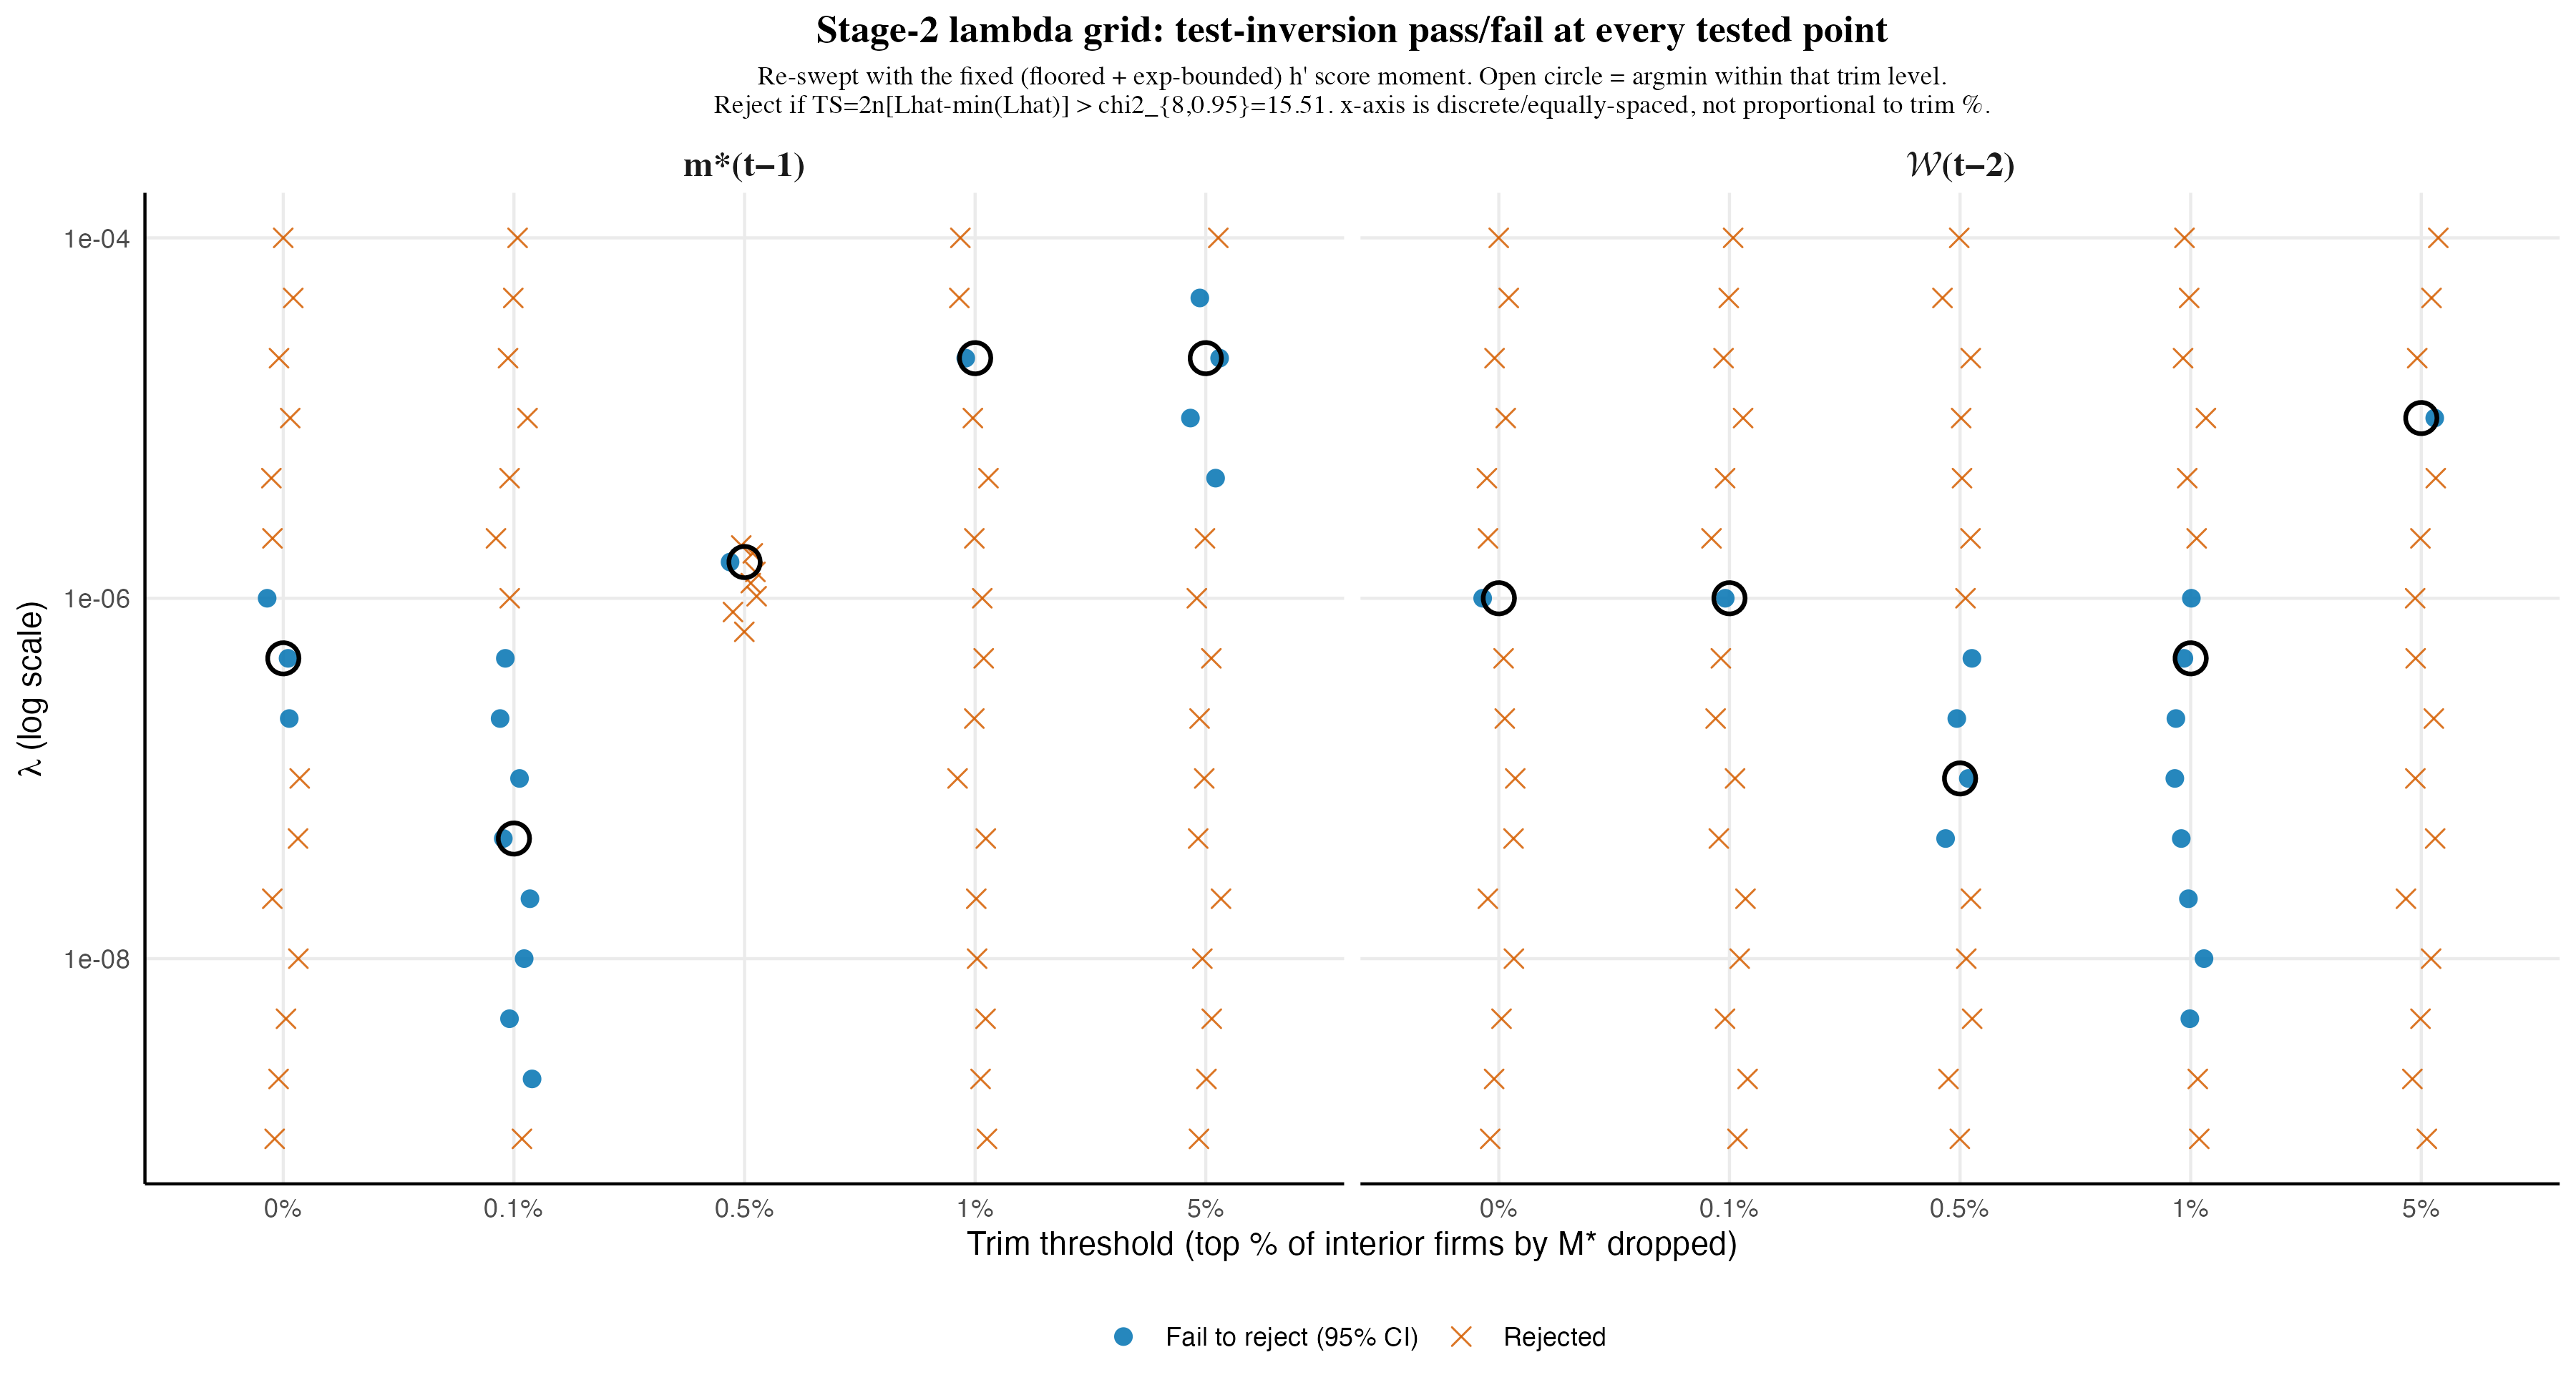
\includegraphics[keepaspectratio]{figures/ch08-trim-cutoff.png}}

}

\caption{\label{fig-cf-trim}Trim-cutoff test inversion.}

\end{figure}%

\subsection{\texorpdfstring{Identification of
\(\lambda\)}{Identification of \textbackslash lambda}}\label{identification-of-lambda}

\begin{itemize}
\tightlist
\item
  From how evasion responds to \(\tau_P\rho_t\) across sector-time
  cells.
\item
  \((\delta_1,\delta_2)\) are pinned by whole-sample linear moments;
  \(\lambda\) only by the curvature of \(\ln(1-2\lambda e)\) through the
  score moment, informative mostly for firms near the ceiling. Say this
  candidly; it explains why \(\lambda\) is the harder parameter.
\end{itemize}

\subsection{Estimates}\label{sec-cf-estimates}

\begin{itemize}
\tightlist
\item
  Search order: \(\lambda\)-grid (profiling \(\delta\)'s), then
  \((\delta_1,\delta_2)\)-grid, then a joint 27-cell
  \((\lambda,\delta_1,\delta_2)\) cube.
\end{itemize}

\begin{figure}

\centering{

\pandocbounded{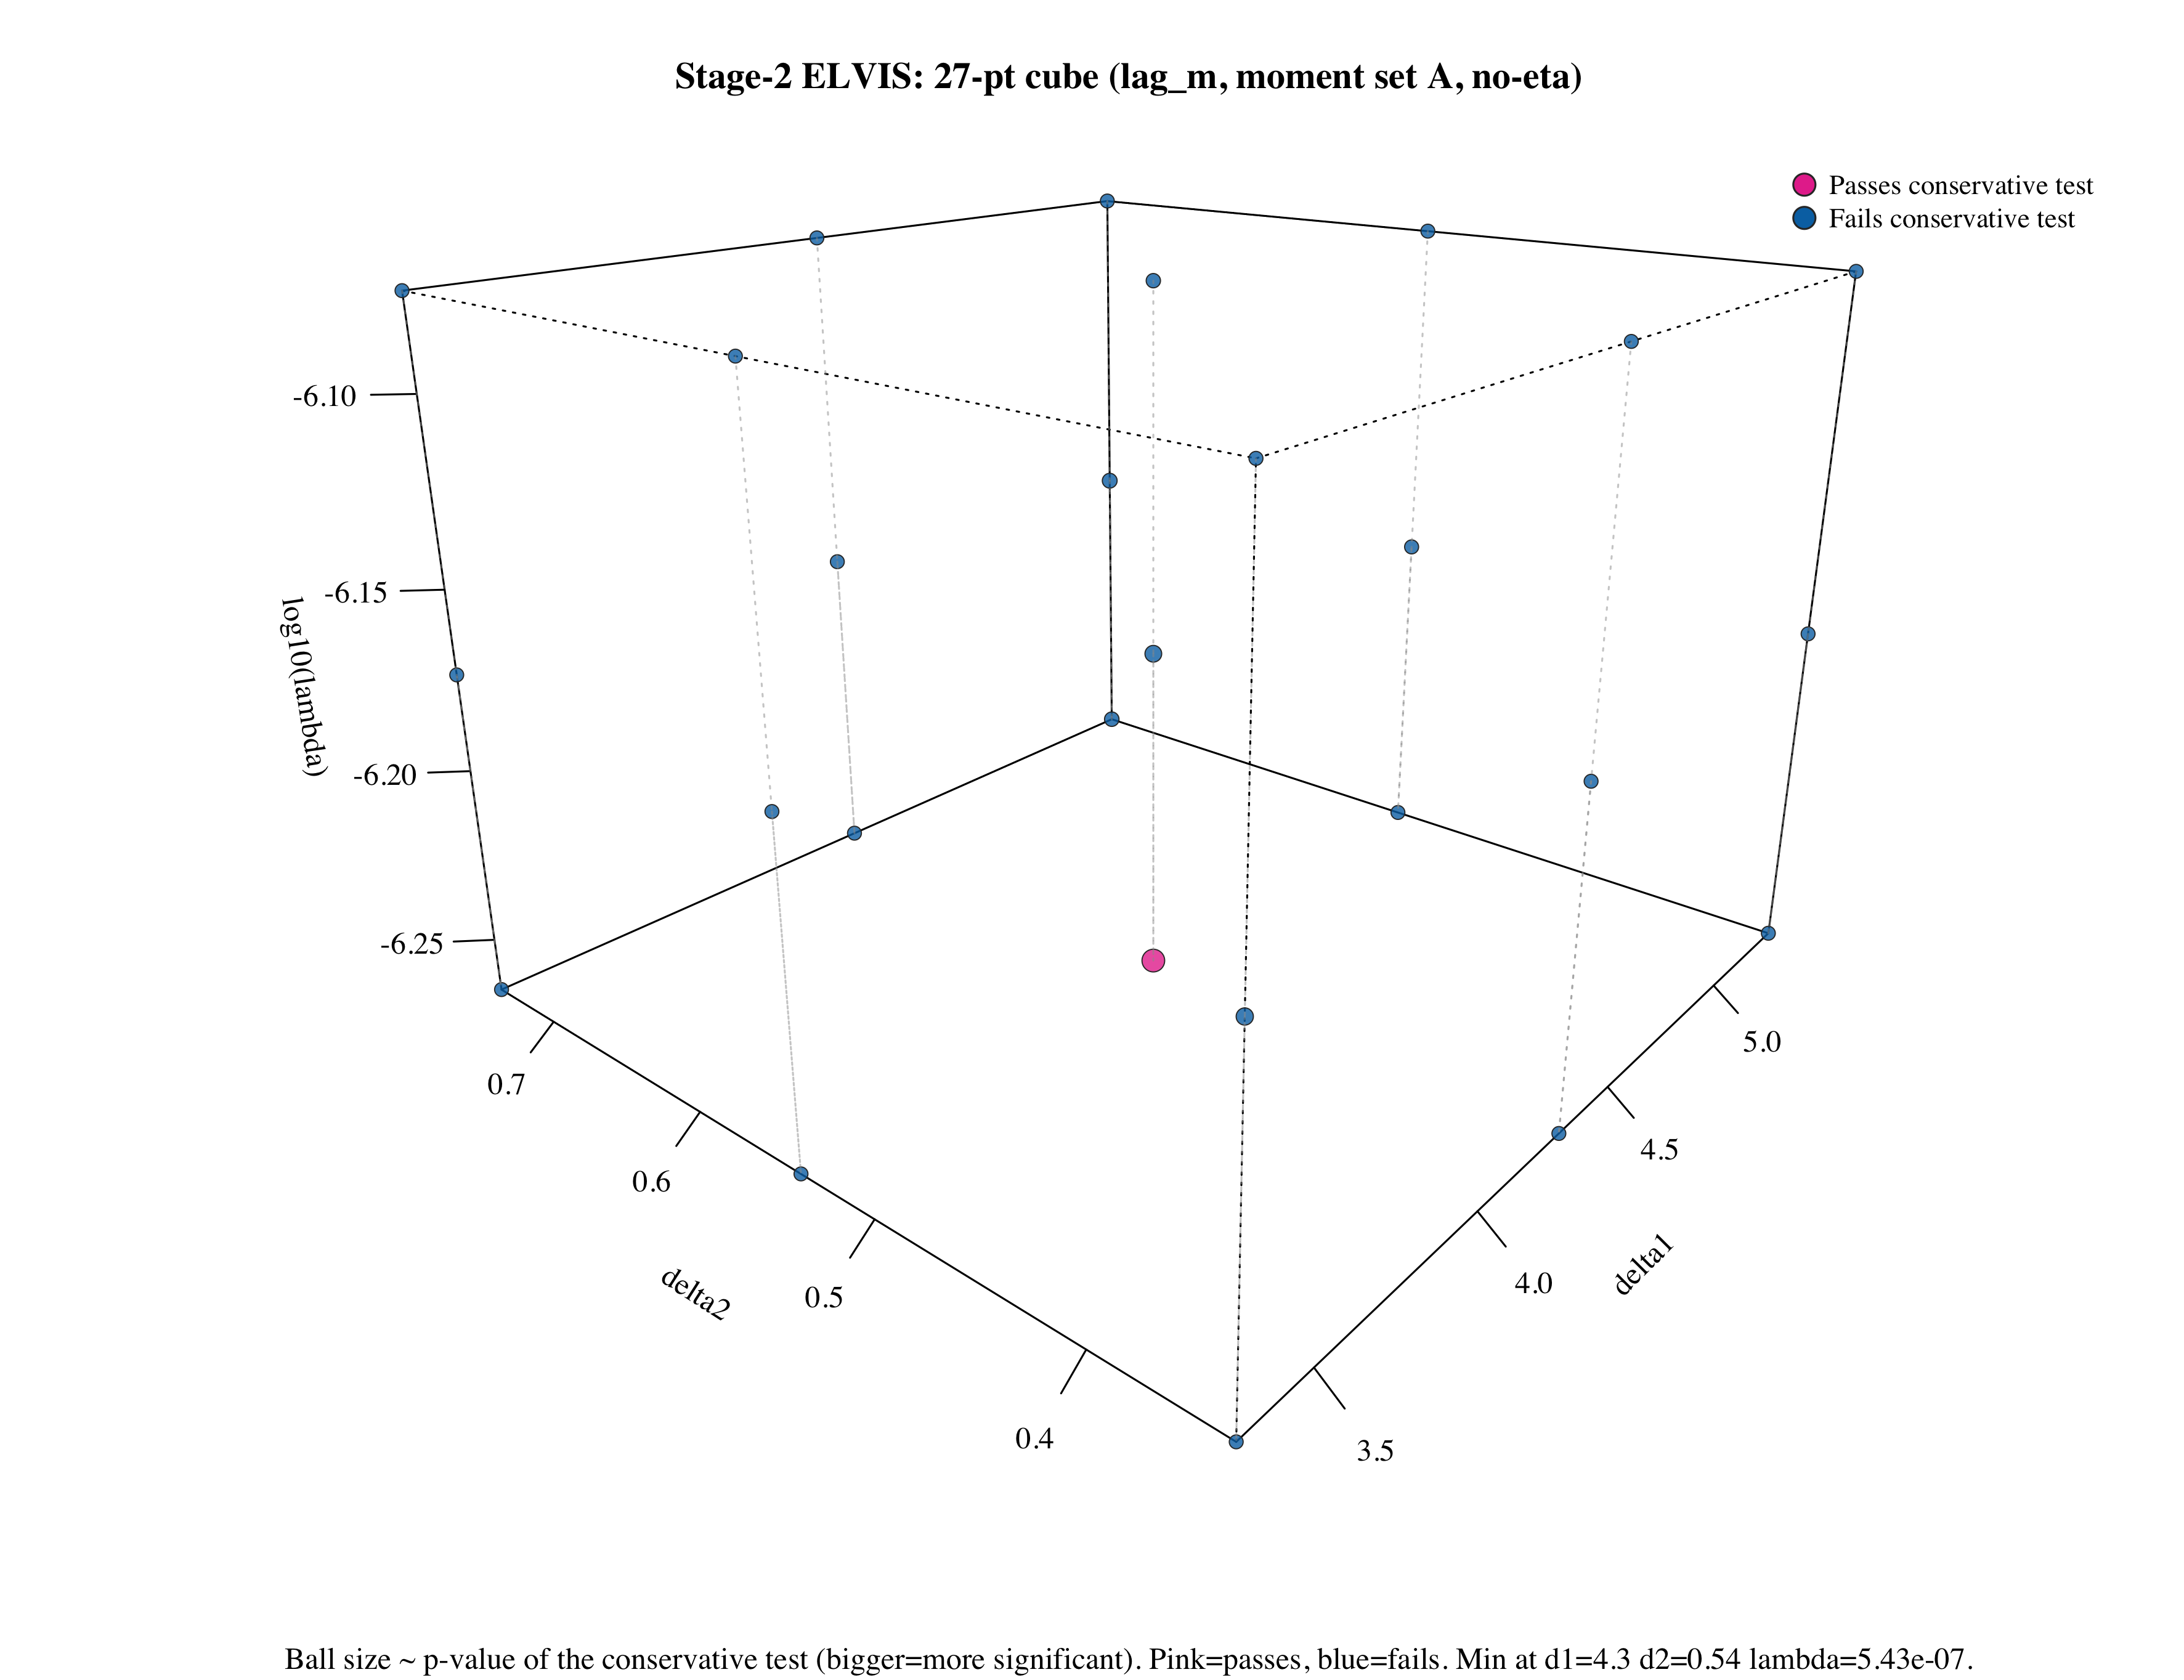
\includegraphics[keepaspectratio]{figures/ch08-elvis-cube.png}}

}

\caption{\label{fig-cf-cube}Joint \((\lambda,\delta_1,\delta_2)\) cube.}

\end{figure}%

\begin{figure}

\centering{

\pandocbounded{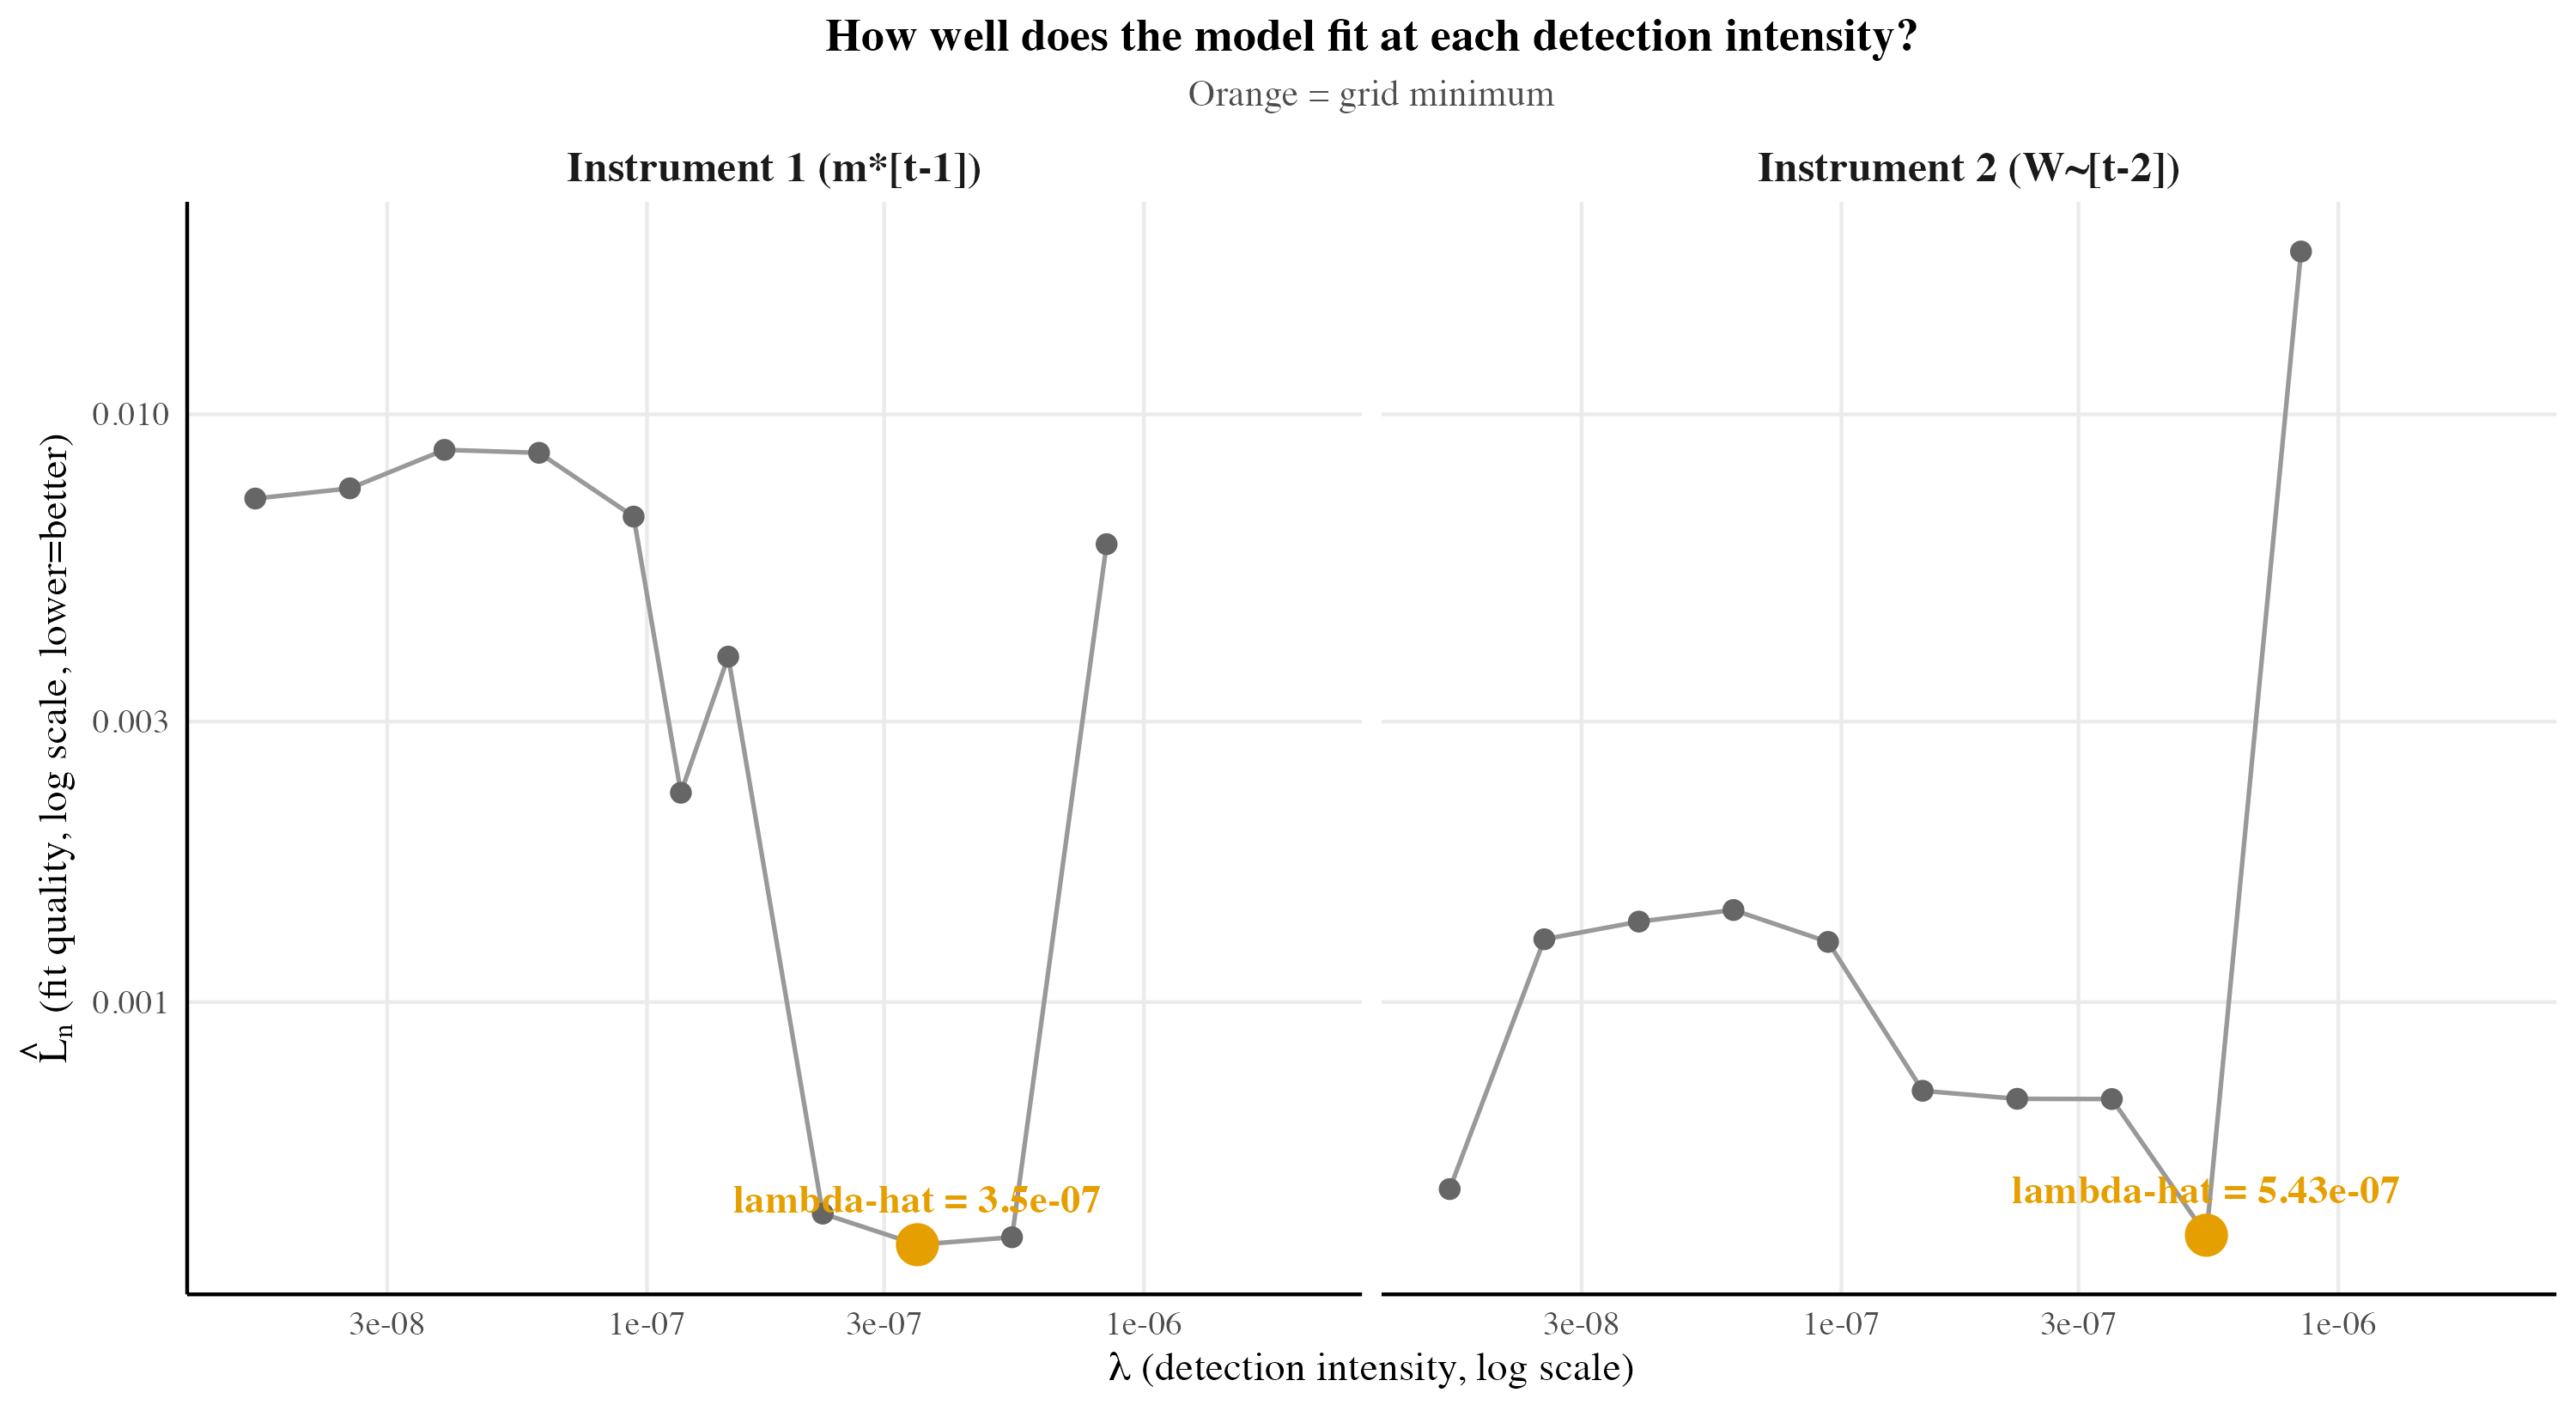
\includegraphics[keepaspectratio]{figures/ch08-lambda-grid.png}}

}

\caption{\label{fig-cf-lambda}\(\lambda\)-grid.}

\end{figure}%

\begin{figure}

\centering{

\pandocbounded{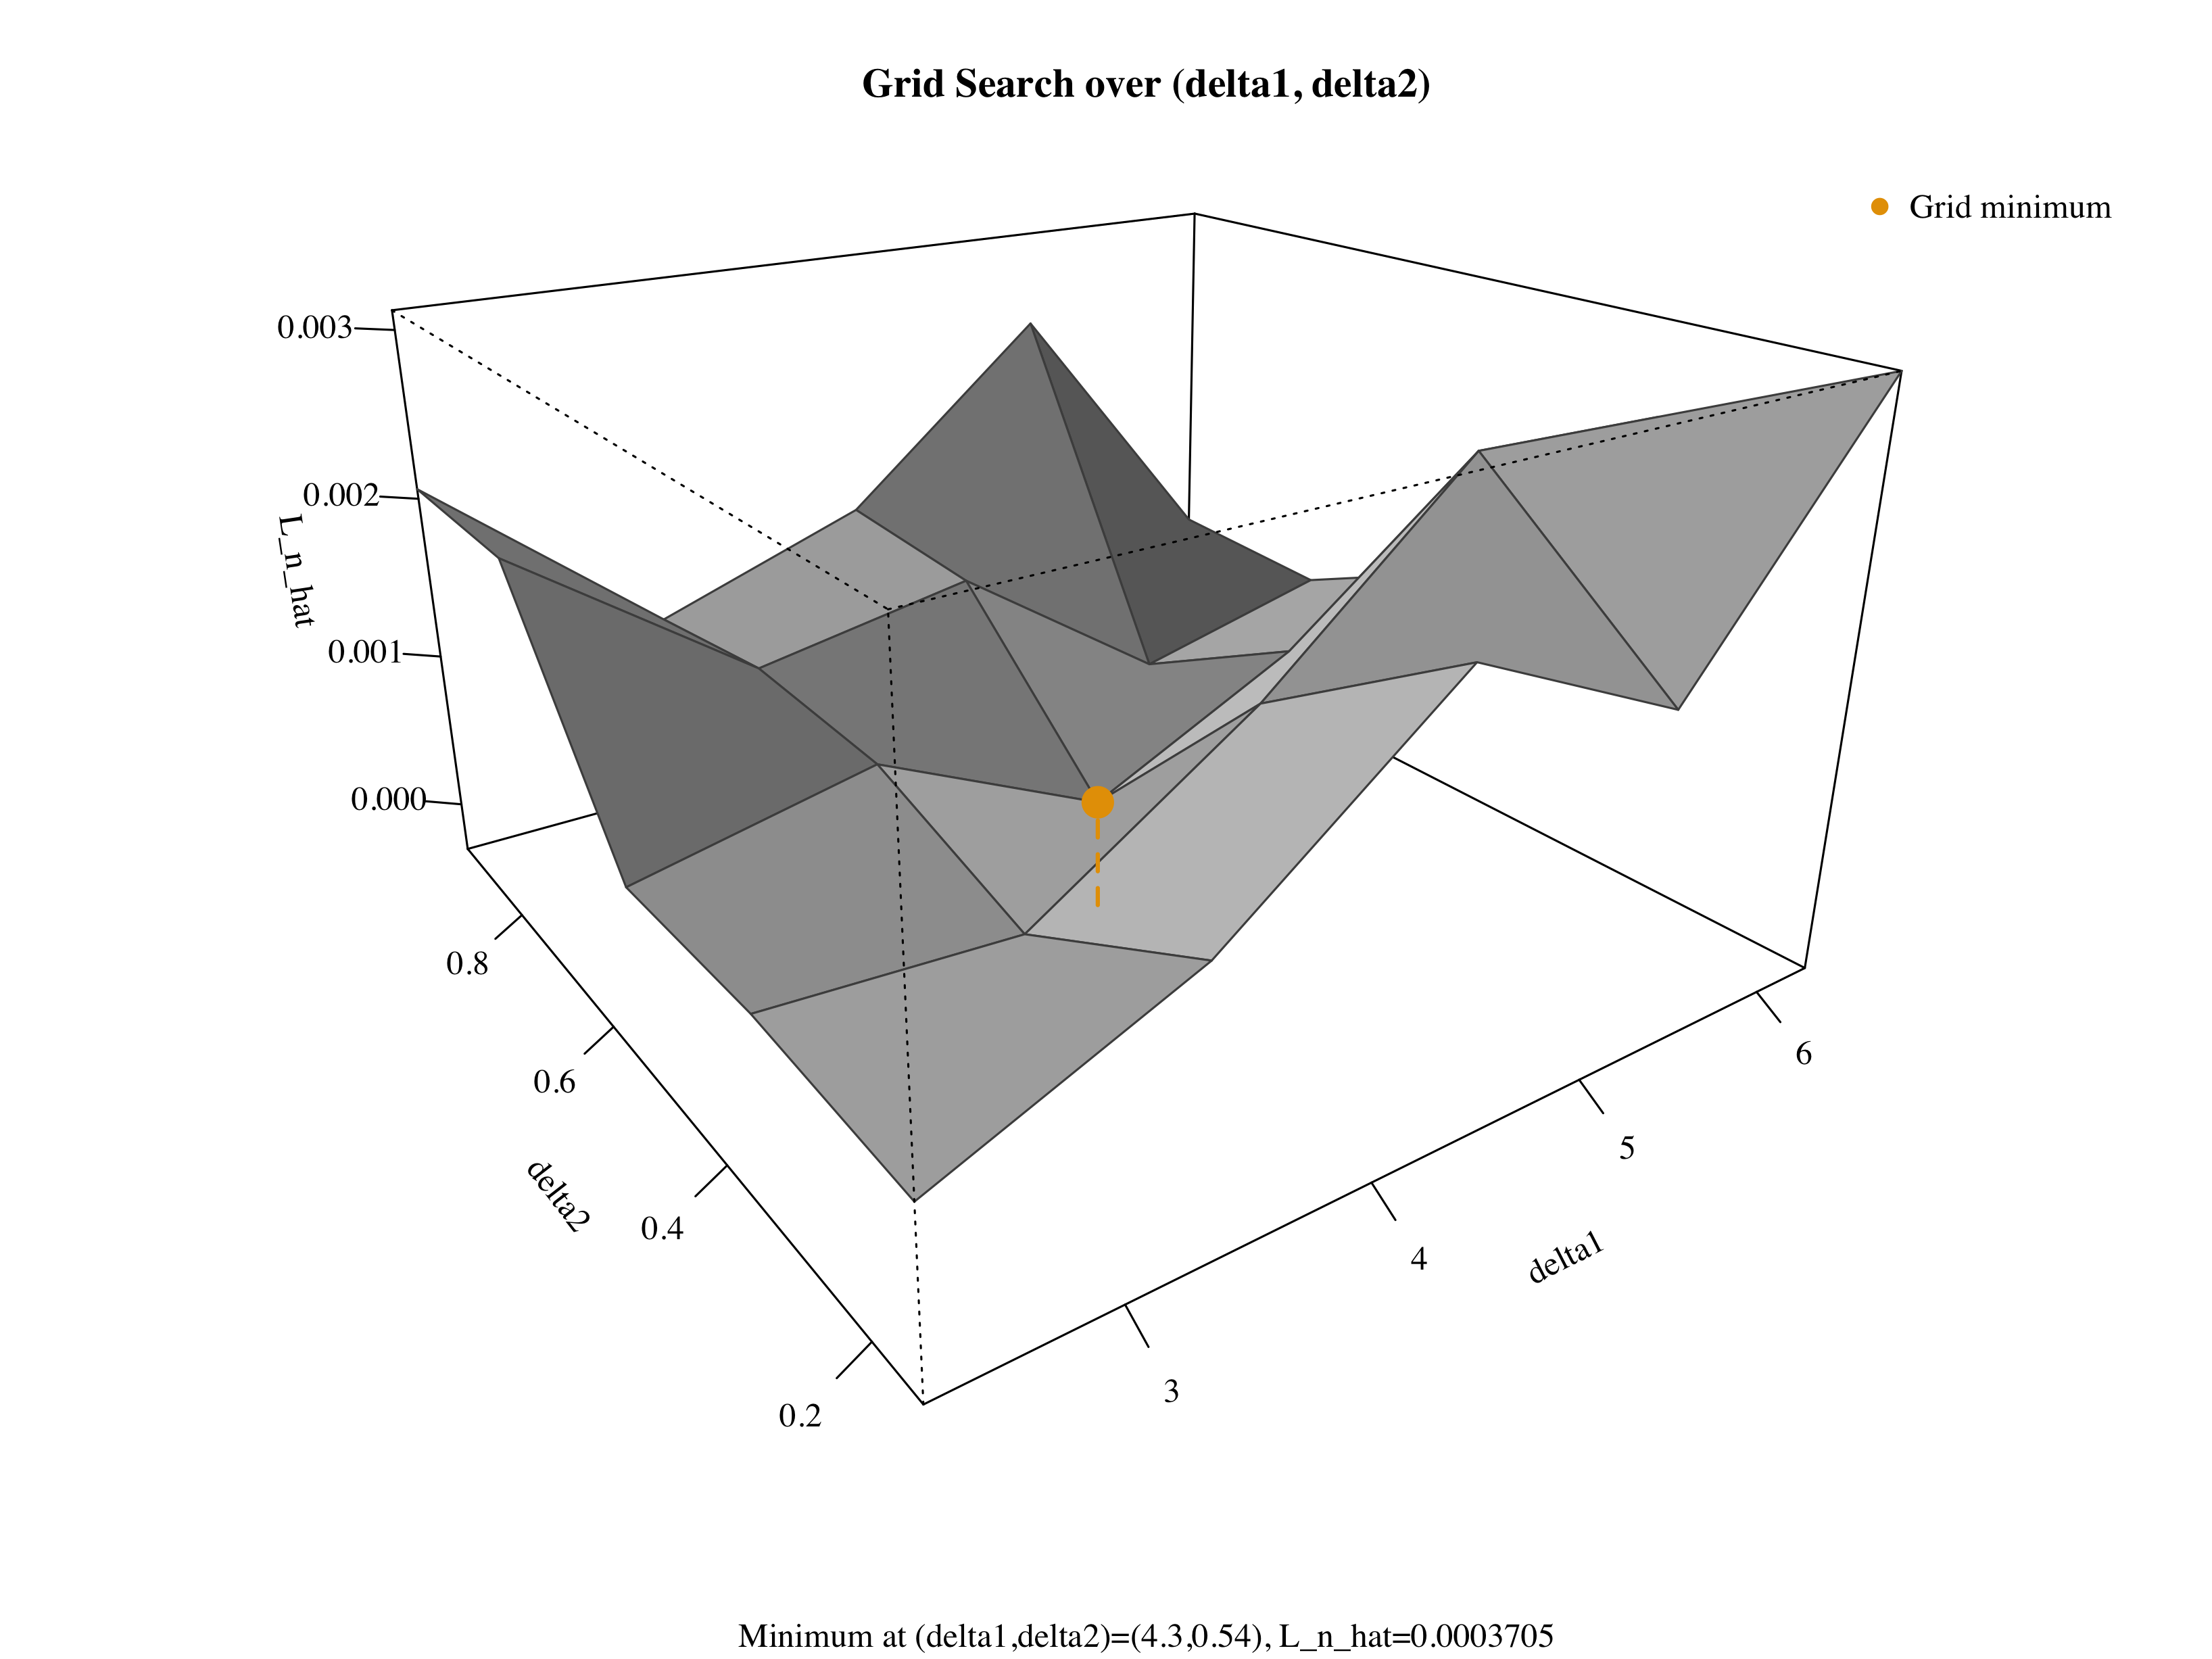
\includegraphics[keepaspectratio]{figures/ch08-delta-grid.png}}

}

\caption{\label{fig-cf-delta}\((\delta_1,\delta_2)\)-grid.}

\end{figure}%

\begin{itemize}
\tightlist
\item
  Best point, \(m^*_{it-1}\) instrument:
  \(\hat\lambda=5.427\times10^{-7}\),
  \((\hat\delta_0,\hat\delta_1,\hat\delta_2)=(3.464,4.300,0.540)\),
  \(\hat\omega^*=3.981\), \(\hat L_n=0.000215\),
  \(TS_{hard}=13.86<16.92\) (passes). 8 of 27 cube cells pass the soft
  test; 4 of 27 also pass the hard test.
\item
  \(\tilde{\mathcal W}_{it-2}\) instrument:
  \(\hat\lambda=5.43\times10^{-7}\), \((10.206,7.460,0.972)\),
  \(\hat\omega^*=3.839\), \(TS_{hard}=25.87\) (fails). Different
  first-stage residuals imply different \(\omega\) distributions, so
  different \(\delta\)'s are expected. Headline uses \(m^*_{it-1}\).
\end{itemize}

\begin{table}

\caption{\label{tbl-cf-estimates}}

\centering{

\pandocbounded{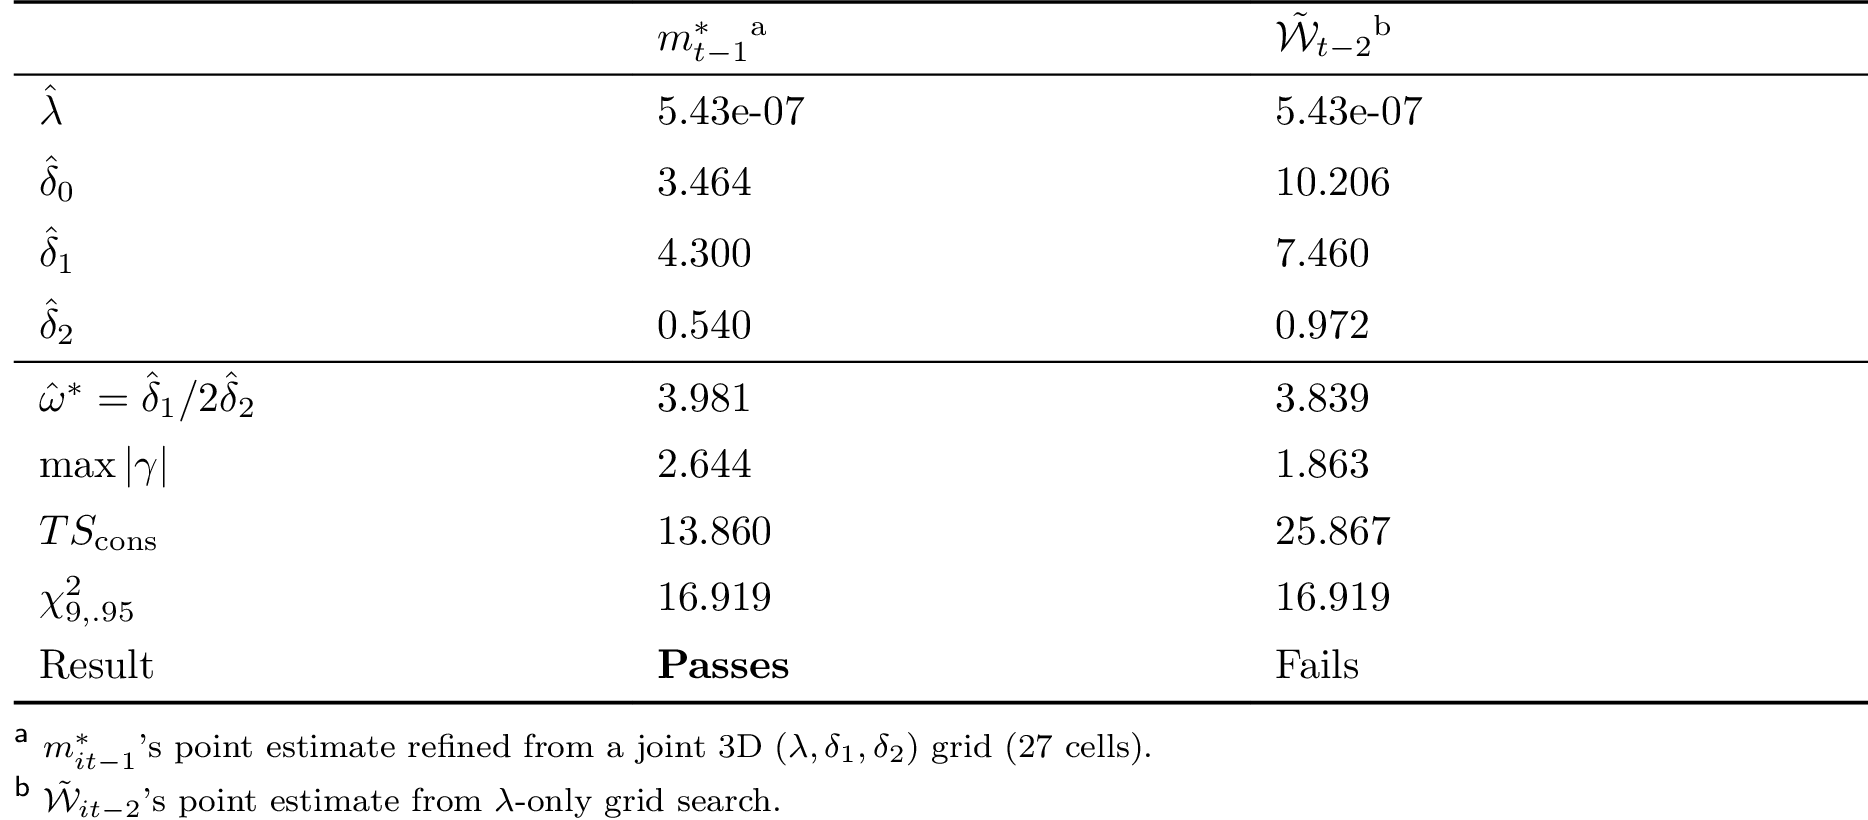
\includegraphics[keepaspectratio]{tables/ch08-headline-estimates.png}}

}

\end{table}%

\begin{itemize}
\tightlist
\item
  Interpretation:

  \begin{itemize}
  \tightlist
  \item
    Cost function has the expected U-shape
    (\(\hat\delta_1,\hat\delta_2>0\) in this parametrization), minimum
    at \(\hat\omega^*=3.98\) (86th percentile, forward simulation).
  \item
    Detection is weak: \(1/(2\hat\lambda)\approx\) \$920,000 versus
    median \(M^*\approx\) \$8,414, P95 \$128,154, P99 \$360,676, largest
    (trimmed) \$701,130.
  \item
    Report detection in relative terms: the P99 evader is about 41-55x
    as likely to be caught as the median evader, whatever
    \(\hat\lambda\) is.
  \end{itemize}
\end{itemize}

\begin{table}

\caption{\label{tbl-cf-detection}}

\centering{

\pandocbounded{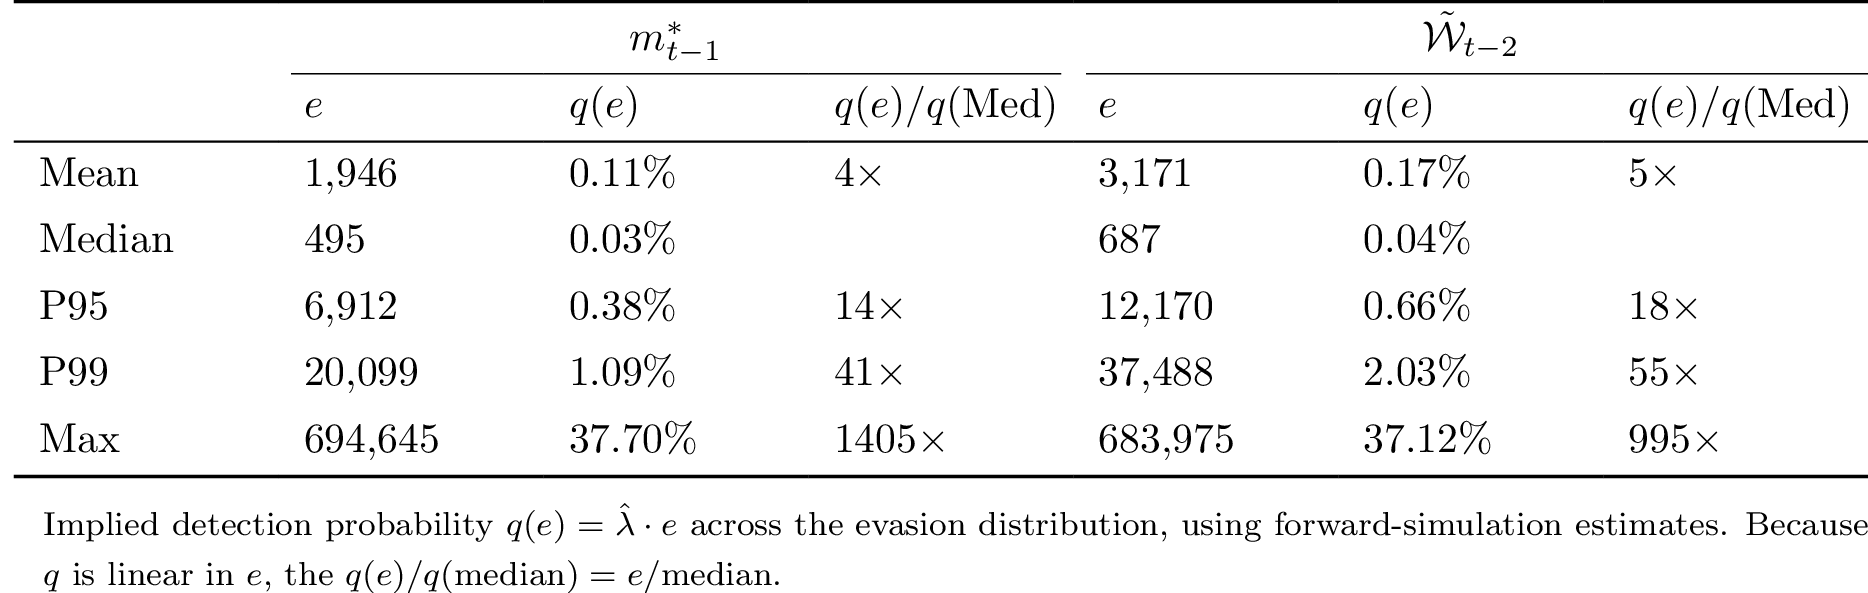
\includegraphics[keepaspectratio]{tables/ch08-detection-prob.png}}

}

\end{table}%

\section{Counterfactual design}\label{sec-cf-design}

\begin{itemize}
\tightlist
\item
  Closed form under linear \(q\), linear \(\kappa\):
  \(\tilde e_i(\Delta)=\max\!\big(0,\frac{e_i+\Delta/(2\lambda)}{1+\Delta}\big)\).
  Slope \(1/(1+\Delta)\) on the firm's own \(e_i\) plus an intercept
  identical across firms. The \(\max(0,\cdot)\) clip is required.
\item
  Counterfactual quantity is a function of the same latent \(M_i\) as
  the main system (not a ``recovered type held fixed''; Schennach 2022
  warns against reading the tilted distribution as the true one).
\item
  Auxiliary parameter \(R(\Delta)\) with its own moment
  \(E[R_i(\Delta;M_i)-R]=0\); \(d_g=10\).
\item
  \(\theta\) is fixed at the best point; only \(\gamma\) is free at each
  \((\Delta,R)\) cell. Question answered: given our best estimates, is a
  candidate revenue consistent with the data? Precedent: Aguiar and
  Kashaev (2020) fix their support parameter in their counterfactual;
  Nail Kashaev endorsed this for the exercise's scope.
\item
  Inference: test inversion. Grid over candidate \(R\) at each
  \(\Delta\); confidence set \(=\{R: TS(\Delta,R)<\chi^2_{10,.95}\}\),
  hard test.
\item
  Control variate (efficiency, not bias): the raw revenue moment has SE
  about \$559 because of firm-size heterogeneity in \(t1_i\). Replace
  with
  \(g^{adj}_{R,i}=\big[R_i(\Delta)/pgdp_i-\hat\beta\,t1_i/pgdp_i\big]-\big[R-\hat\beta\mu_c\big]\),
  \(\hat\beta=0.998838\), \(\mu_c=E[t1_i/pgdp_i]=2507.60\) (both fixed
  constants). \(E[g^{adj}]=E[g]\) exactly; SE falls from about \$559 to
  about \$14 (38-41x). Industry x year fixed effects only reach 2.5x
  (additive: \$559 to \$508; full interaction: \$223, 318 nuisance
  cells, 100 with \textless30 obs).
\item
  Expected details for the appendix: derivation and validity proof in
  \texttt{9999-control-variate.qmd}.
\end{itemize}

\section{Results}\label{sec-cf-results}

\begin{figure}

\centering{

\pandocbounded{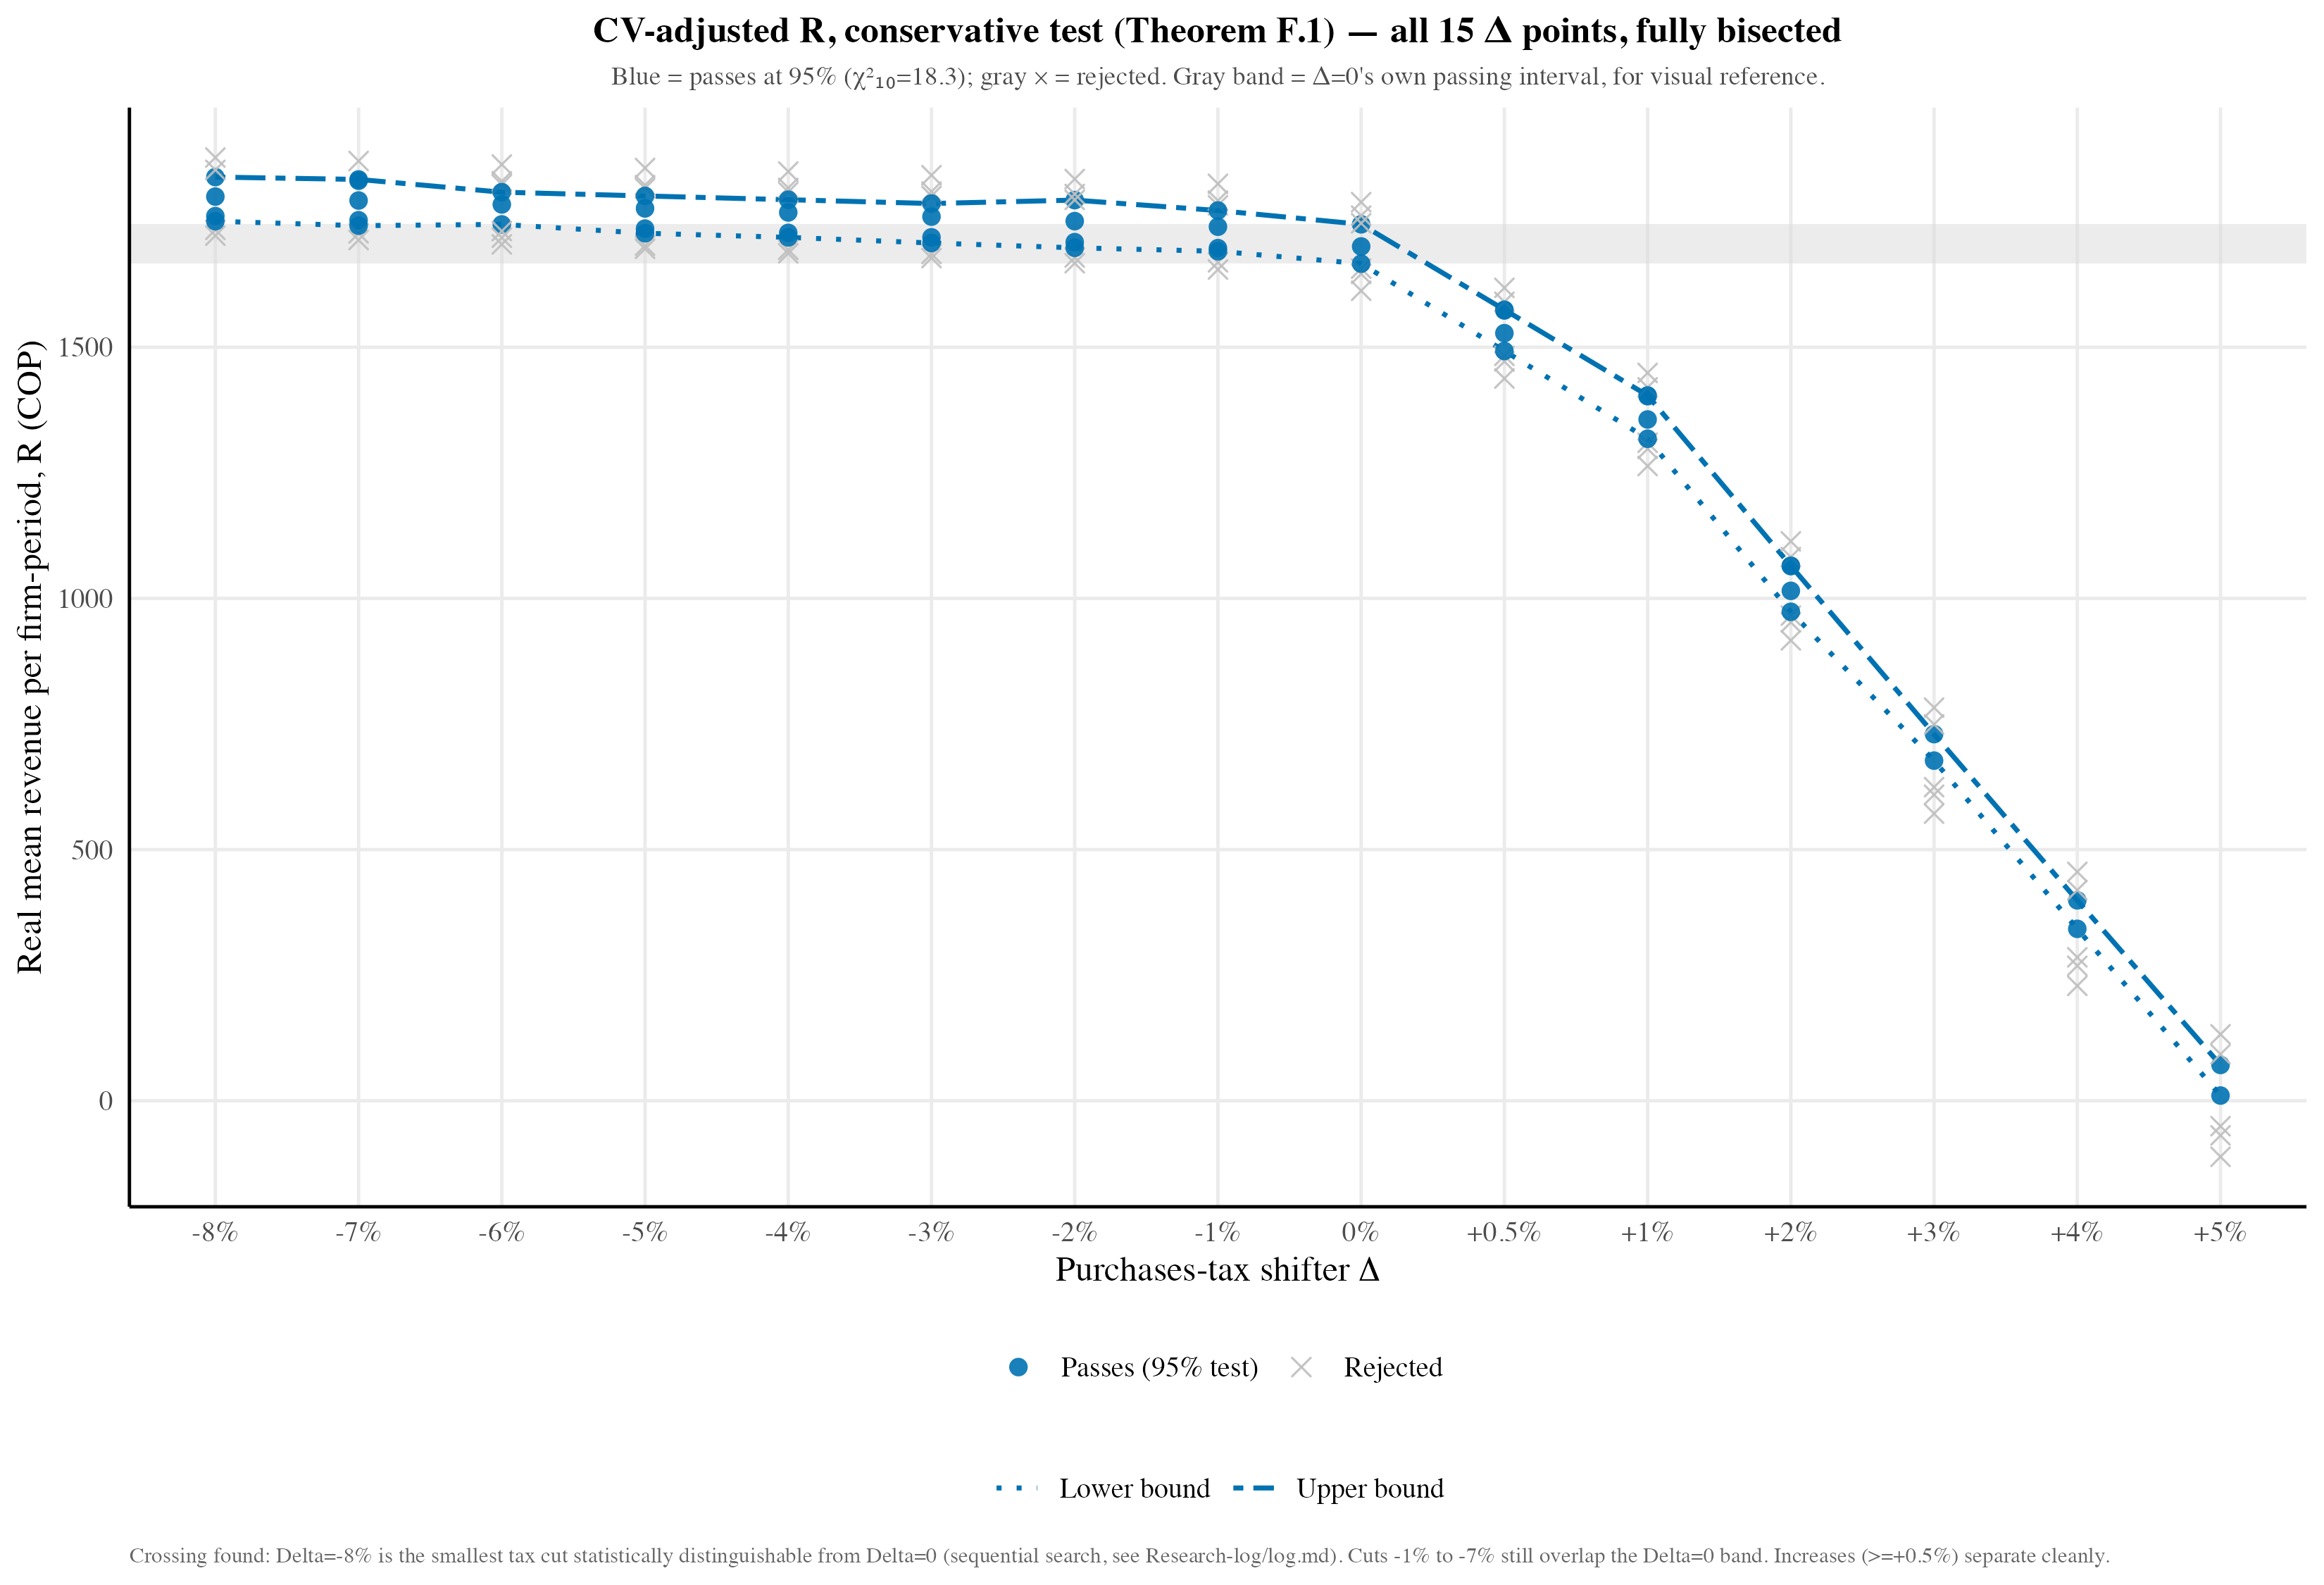
\includegraphics[keepaspectratio]{figures/ch08-laffer-ci-hard.png}}

}

\caption{\label{fig-cf-laffer}Hard-test 95\% confidence sets for real
mean revenue by \(\Delta\); gray band = current policy's interval.}

\end{figure}%

\begin{itemize}
\tightlist
\item
  Real mean revenue per firm-period, 95\% hard-test CIs:
\end{itemize}

{\def\LTcaptype{none} % do not increment counter
\begin{longtable}[]{@{}
  >{\raggedleft\arraybackslash}p{(\linewidth - 30\tabcolsep) * \real{0.0625}}
  >{\raggedleft\arraybackslash}p{(\linewidth - 30\tabcolsep) * \real{0.0625}}
  >{\raggedleft\arraybackslash}p{(\linewidth - 30\tabcolsep) * \real{0.0625}}
  >{\raggedleft\arraybackslash}p{(\linewidth - 30\tabcolsep) * \real{0.0625}}
  >{\raggedleft\arraybackslash}p{(\linewidth - 30\tabcolsep) * \real{0.0625}}
  >{\raggedleft\arraybackslash}p{(\linewidth - 30\tabcolsep) * \real{0.0625}}
  >{\raggedleft\arraybackslash}p{(\linewidth - 30\tabcolsep) * \real{0.0625}}
  >{\raggedleft\arraybackslash}p{(\linewidth - 30\tabcolsep) * \real{0.0625}}
  >{\raggedleft\arraybackslash}p{(\linewidth - 30\tabcolsep) * \real{0.0625}}
  >{\raggedleft\arraybackslash}p{(\linewidth - 30\tabcolsep) * \real{0.0625}}
  >{\raggedleft\arraybackslash}p{(\linewidth - 30\tabcolsep) * \real{0.0625}}
  >{\raggedleft\arraybackslash}p{(\linewidth - 30\tabcolsep) * \real{0.0625}}
  >{\raggedleft\arraybackslash}p{(\linewidth - 30\tabcolsep) * \real{0.0625}}
  >{\raggedleft\arraybackslash}p{(\linewidth - 30\tabcolsep) * \real{0.0625}}
  >{\raggedleft\arraybackslash}p{(\linewidth - 30\tabcolsep) * \real{0.0625}}
  >{\raggedleft\arraybackslash}p{(\linewidth - 30\tabcolsep) * \real{0.0625}}@{}}
\toprule\noalign{}
\begin{minipage}[b]{\linewidth}\raggedleft
\(\Delta\)
\end{minipage} & \begin{minipage}[b]{\linewidth}\raggedleft
\(-8\%\)
\end{minipage} & \begin{minipage}[b]{\linewidth}\raggedleft
\(-7\%\)
\end{minipage} & \begin{minipage}[b]{\linewidth}\raggedleft
\(-6\%\)
\end{minipage} & \begin{minipage}[b]{\linewidth}\raggedleft
\(-5\%\)
\end{minipage} & \begin{minipage}[b]{\linewidth}\raggedleft
\(-4\%\)
\end{minipage} & \begin{minipage}[b]{\linewidth}\raggedleft
\(-3\%\)
\end{minipage} & \begin{minipage}[b]{\linewidth}\raggedleft
\(-2\%\)
\end{minipage} & \begin{minipage}[b]{\linewidth}\raggedleft
\(-1\%\)
\end{minipage} & \begin{minipage}[b]{\linewidth}\raggedleft
\(0\%\)
\end{minipage} & \begin{minipage}[b]{\linewidth}\raggedleft
\(+0.5\%\)
\end{minipage} & \begin{minipage}[b]{\linewidth}\raggedleft
\(+1\%\)
\end{minipage} & \begin{minipage}[b]{\linewidth}\raggedleft
\(+2\%\)
\end{minipage} & \begin{minipage}[b]{\linewidth}\raggedleft
\(+3\%\)
\end{minipage} & \begin{minipage}[b]{\linewidth}\raggedleft
\(+4\%\)
\end{minipage} & \begin{minipage}[b]{\linewidth}\raggedleft
\(+5\%\)
\end{minipage} \\
\midrule\noalign{}
\endhead
\bottomrule\noalign{}
\endlastfoot
lower & 1751 & 1742 & 1744 & 1727 & 1719 & 1707 & 1698 & 1691 & 1666 &
1492 & 1318 & 973 & 677 & 342 & 10 \\
upper & 1839 & 1834 & 1809 & 1801 & 1794 & 1786 & 1793 & 1772 & 1745 &
1575 & 1404 & 1065 & 730 & 399 & 71 \\
\end{longtable}
}

\begin{itemize}
\tightlist
\item
  Headline (Table~\ref{tbl-cf-headline}): a tax increase of 0.5\% is
  already statistically distinguishable from current policy; a cut
  raises revenue but only becomes distinguishable at -8\% (crossing
  located by sequential search: -10\%, -9\%, -8\% separate, -7\% does
  not).

  \begin{itemize}
  \tightlist
  \item
    Baseline CI \([1666,1745]\). Cut of 8\%: \([1751,1839]\), guaranteed
    change +0.35\% to +10.34\%, point +5.84\%. Increase of 0.5\%:
    \([1492,1575]\), guaranteed -14.45\% to -5.50\%, point -10.15\%.
  \item
    Result is a set, not a point \(\tau^*\); state this as the
    deliverable, not a fallback.
  \end{itemize}
\end{itemize}

\begin{table}

\caption{\label{tbl-cf-headline}}

\centering{

\pandocbounded{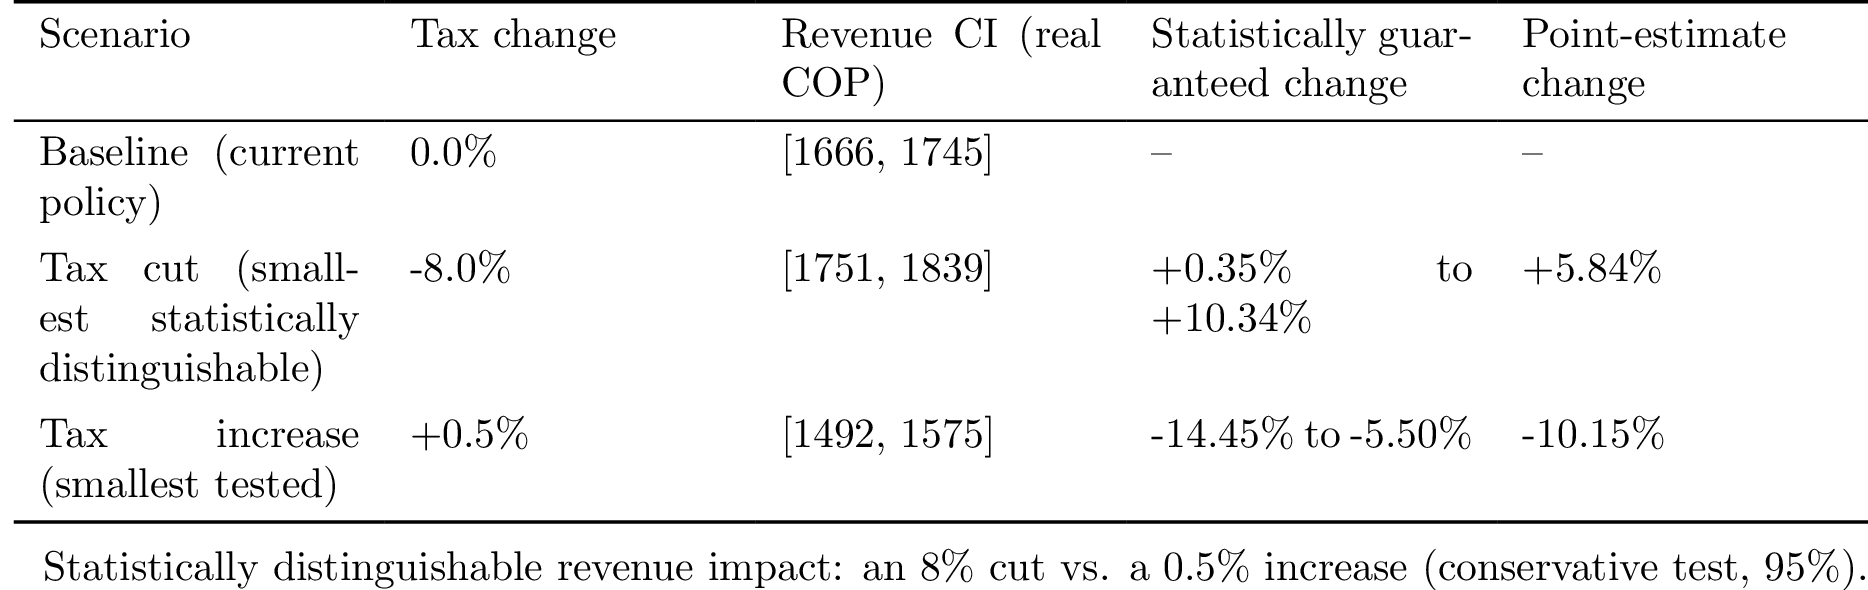
\includegraphics[keepaspectratio]{tables/ch08-headline-pct.png}}

}

\end{table}%

\begin{itemize}
\tightlist
\item
  Mechanism for the asymmetry:
  \(\tilde e(\Delta)=[e_i+\Delta/(2\lambda)]/(1+\Delta)\) is a horse
  race between \(e_i\) and the common intercept \(\Delta/(2\lambda)\).
  With \(\hat\lambda\) tiny, the intercept wins: an increase shifts
  every firm by about the same large amount; a cut removes evasion firm
  by firm (small evaders hit zero first), so the aggregate response is
  gradual.
\item
  This is a property of linear \(q\) and linear \(\kappa\) combined with
  small \(\hat\lambda\), not of linearity alone. Convex
  \(q=(\lambda e)^k\) and concave \(q=1-e^{-\lambda e}\) break the
  uniform-shift result (closed forms derived, not estimated).
\end{itemize}

\section{Robustness}\label{sec-cf-robust}

\begin{itemize}
\tightlist
\item
  \(\theta\) free instead of fixed: at \(\Delta=-4\%\) with \(\theta\)
  free (seeded at the fixed point), \(\hat\theta\) moved 0.1-2\% and
  pass/fail replicated at 4 of 5 candidates, so the tight sets reflect
  cross-firm heterogeneity, not fixing \(\theta\).
\item
  Is the CV precision real? Truncation pattern of \(\hat\Omega^-\) is
  the same for raw and CV revenue (4 of 10 directions kept in both). At
  \(\Delta=-4\%\), \(R=1850\): same deviation (\(\approx\$82\)),
  different yardstick (SE \$559.4 vs.~\$13.5): \(0.15\) SEs vs.~\(6.03\)
  SEs. Efficient weighting working correctly, not a numerical artifact.
\item
  Is \(\hat\beta\) data-mined? Set the coefficient to exactly 1 from the
  revenue identity (\(R_i-t1_i=-\tau_P[M_i+(1-q)e']\)). Every implied CI
  (9 values of \(\Delta\)) nests inside the CV CI (e.g.~\(\Delta=0\):
  \([1701,1745]\) vs.~\([1666,1745]\); \(\Delta=-8\%\): \([1788,1827]\)
  vs.~\([1751,1839]\)).
\end{itemize}

\begin{figure}

\centering{

\pandocbounded{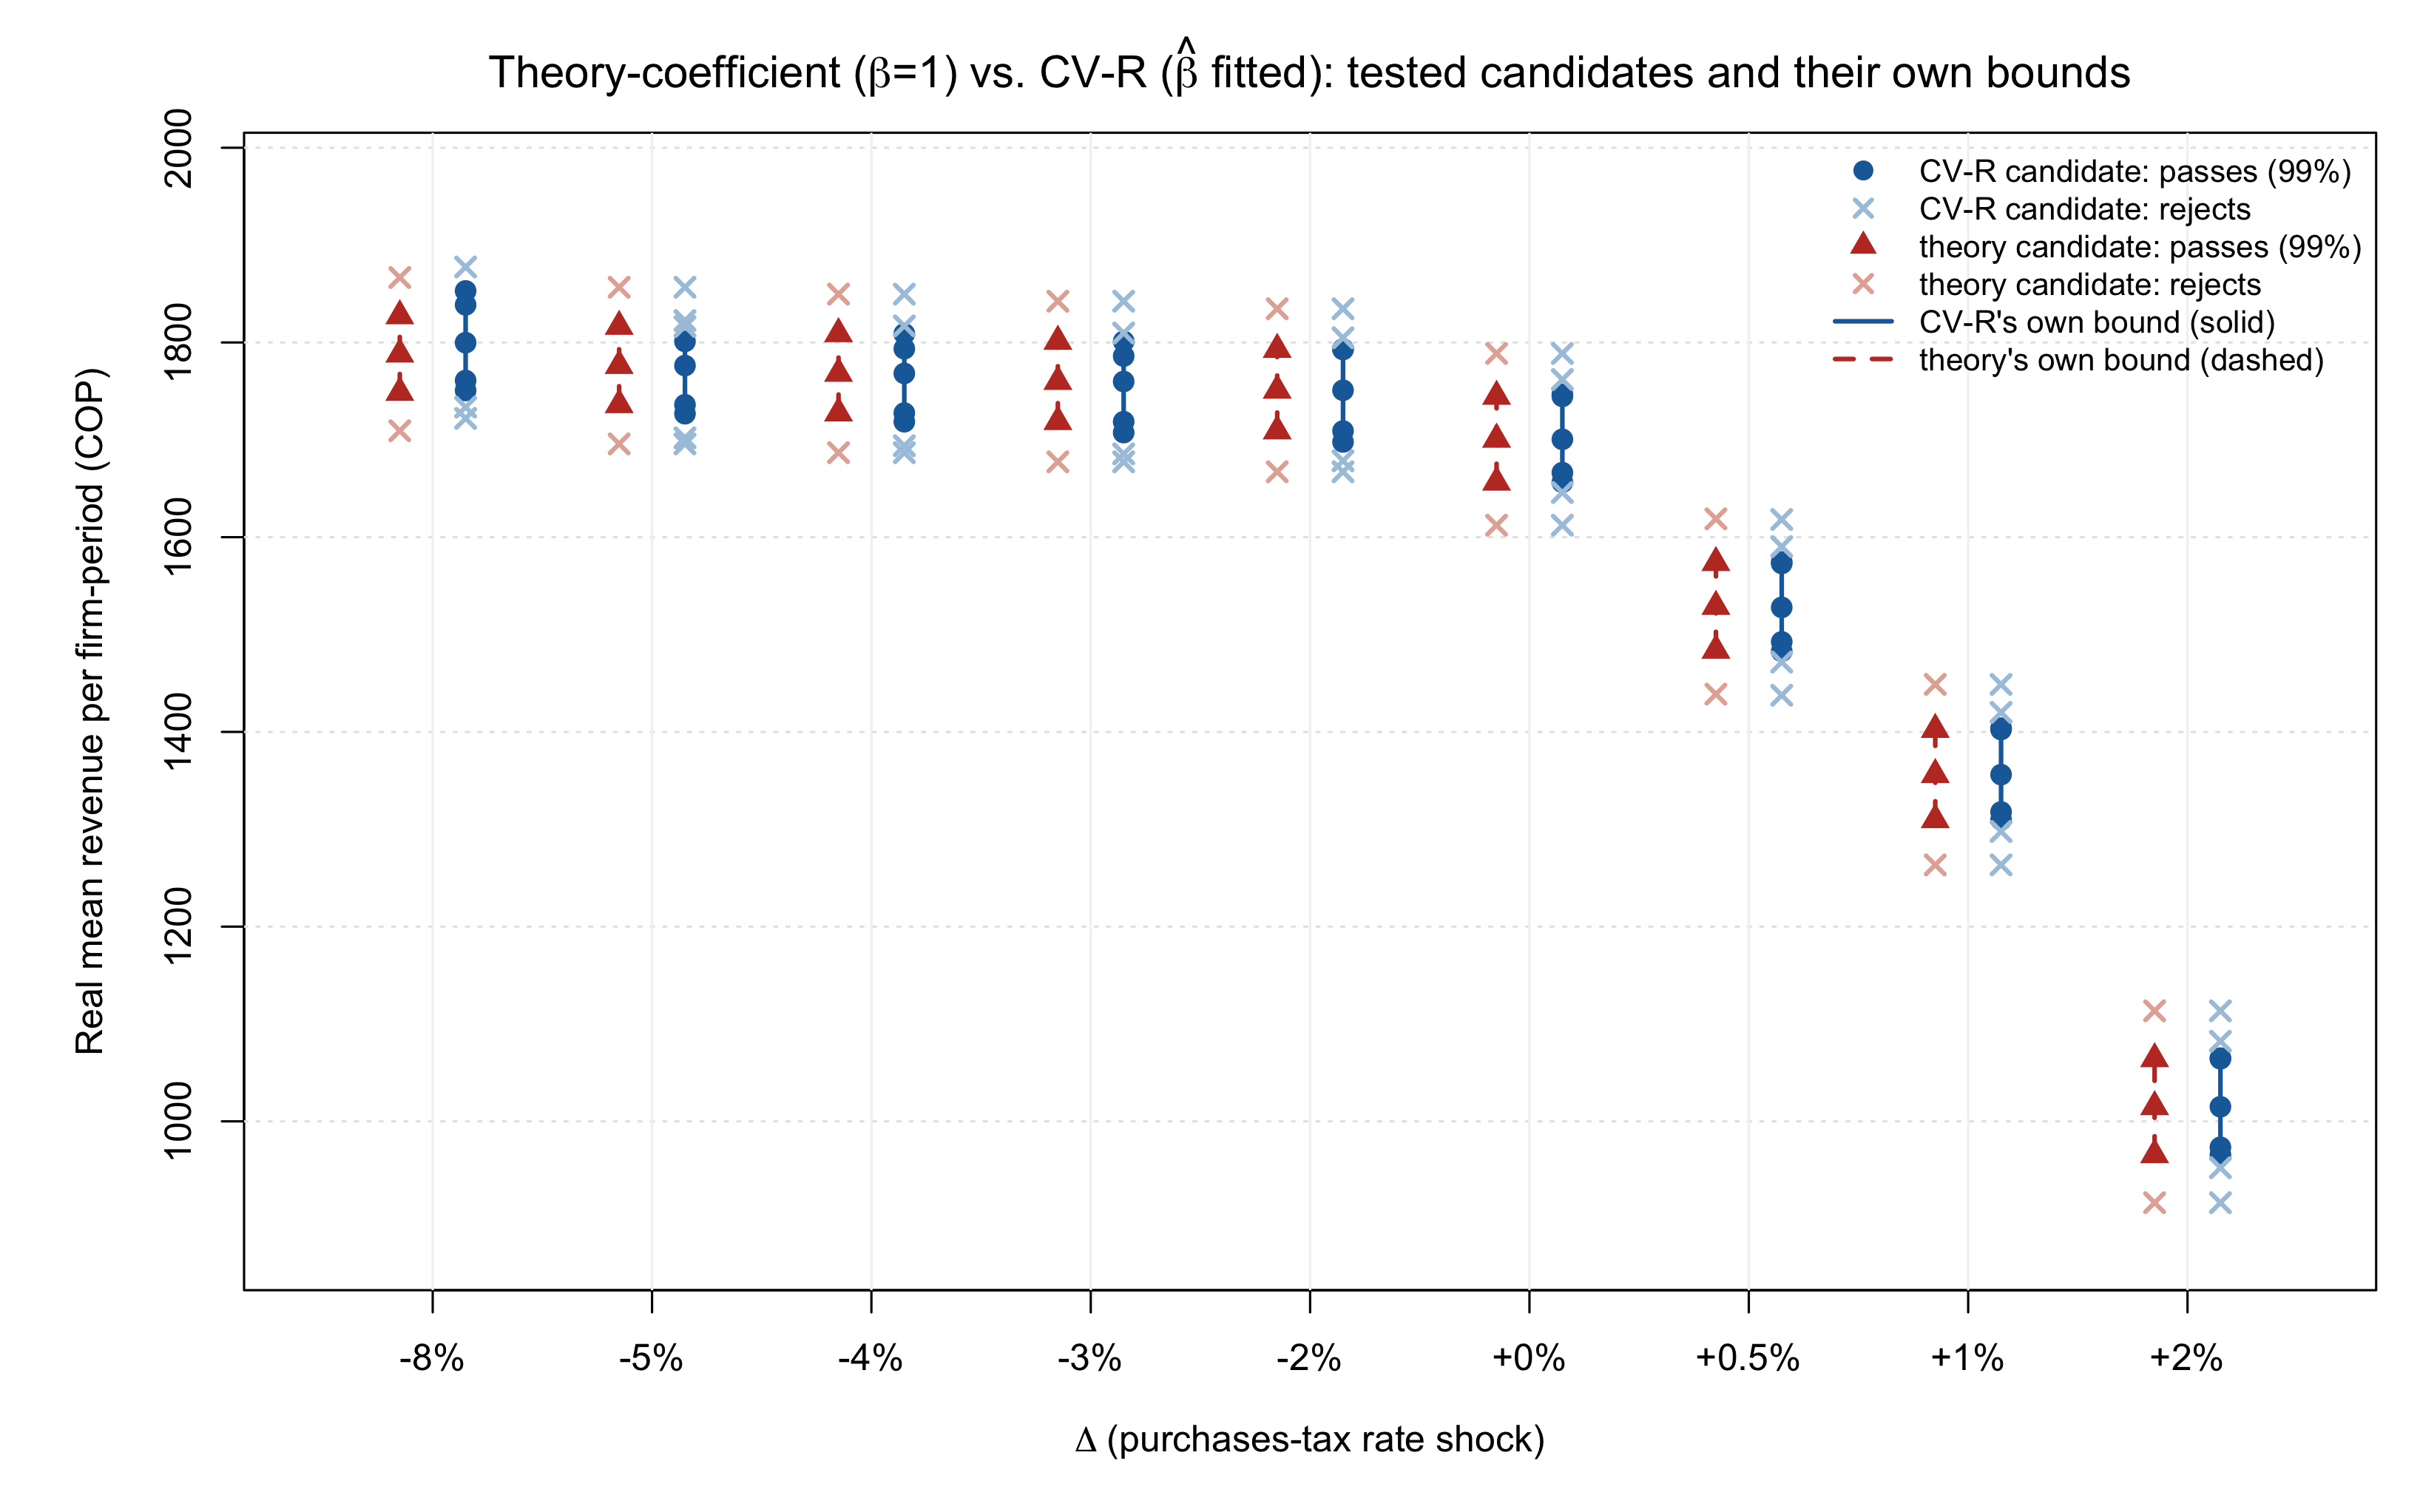
\includegraphics[keepaspectratio]{figures/ch08-theory-vs-cv.png}}

}

\caption{\label{fig-cf-theory-cv}Theory-coefficient vs.~CV passing
points.}

\end{figure}%

\begin{itemize}
\tightlist
\item
  Costs of the variance reduction (state honestly): forcing \(\gamma\)
  to fit a tight \(R\) target inflates the SE of the
  \(\varepsilon\cdot e\) moment (about 5.4x at the tested point); a
  sharper test also rejects on other small misspecifications.
\item
  Rejected alternative: a revenue-loss moment (more degenerate for
  \(\Delta\lesssim-2\%\); most brackets inconclusive).
\item
  Planned (not run): instrument comparison
  (\(\tilde{\mathcal W}_{it-2}\)); cap \(R_i\ge0\) (equivalent to
  capping \(e'\)) at \(+2\%,+4\%,+8\%\), pending Nail Kashaev.
\end{itemize}

\section{Scope and limits}\label{sec-cf-limits}

\begin{itemize}
\tightlist
\item
  Partial equilibrium: \(K\), \(L\), \(\omega\), \(\varepsilon\) and
  \(M\) held fixed; only evasion responds. Large \(\Delta\) is outside
  what the exercise can speak to.
\item
  \(\theta\) fixed at one operating point that is not rejected (hard
  test) for \(m^*_{it-1}\) only; the second instrument does not pass.
\item
  \(\hat\lambda\) is identified mostly from a thin tail of aggressive
  evaders; the estimate depends on the 0.5\% trim.
\item
  Stage 1 is not yet re-estimated with net-of-tax sales and purchases
  (pending supervisor conversation); mention as extension.
\item
  \textbf{MUST STATE EXPLICITLY TO SUPERVISORS, not silently:} the ELVIS
  estimates
  \(\hat\theta=(\hat\lambda,\hat\delta_0,\hat\delta_1,\hat\delta_2)\)
  and everything built on them (the whole counterfactual) inherit
  \(\hat\beta\) from the gross/single-tax first stage, not the
  net-of-tax one -- even though the evasion FOC itself is already
  correctly two-tax (\(h(e)\) uses only \(\tau_P\)). The exposure is the
  \emph{materials-FOC/production-identity} side that feeds
  \(\mathcal V_{it}\)/\(\tilde{\mathcal W}_{it}\), same channel the
  \texttt{1470}/\texttt{1471} diagnostic measured (\(\hat\beta\) moves
  \(-0.006\) on average) -- small, but ELVIS has not itself been re-run
  to confirm it stays small there. Re-running ELVIS on a net-of-tax
  first stage is future work, explicitly NOT scoped for this week.
\end{itemize}

\section{Open items}\label{open-items-2}

\begin{itemize}
\tightlist
\item[$\square$]
  Move figures and tables to \texttt{Code/Thesis/ch08-*.R} scripts
  (currently copied PNGs; producing scripts:
  \texttt{1289-cube-3dplot.R}, \texttt{1305-lambdagrid-minonly-plot.R},
  \texttt{1306-deltagrid-minonly-3dplot.R},
  \texttt{1222-stage2-trim-all-gridpoints-plot.R},
  \texttt{1300-cv-15delta-hard-plot.R},
  \texttt{1301-headline-pct-table.R},
  \texttt{1303-detection-prob-table.R},
  \texttt{1304-headline-estimates-table.R},
  \texttt{1307-theory-vs-cv-plot.R}).
\item[$\square$]
  Add the CI table as a generated PNG
  (\texttt{Code/Thesis/ch08-laffer-ci-table.R}) instead of the markdown
  table above.
\item[$\square$]
  Decide whether the pure-simulation Laffer curve (\texttt{1279},
  \texttt{1280}) appears (point estimates only: 1\% cut +3.51\%, next
  1\% +0.77\%, 0.1\% increase -3.13\%); formal inference does not
  separate adjacent \(\Delta\)'s at that resolution.
\item[$\square$]
  Write the stage-2 appendix (ELVIS derivation, MSL and naive-MSM
  rejection, cross-test table \texttt{1444}).
\end{itemize}

\bookmarksetup{startatroot}

\chapter{Related Literature}\label{sec-literature}

\bookmarksetup{startatroot}

\chapter{Conclusion}\label{sec-conclusion}

\cleardoublepage
\phantomsection
\addcontentsline{toc}{part}{Appendices}
\appendix

\chapter{ELVIS Derivation and the MSM/MSL
Alternatives}\label{sec-app-elvis}

\chapter{Control-Variate Correction}\label{sec-app-cv}

\chapter{MSL Implementation and Density
Transformation}\label{sec-app-msl}

\protect\phantomsection\label{refs}
\begin{CSLReferences}{1}{1}
\bibitem[\citeproctext]{ref-Allingham1972}
Allingham, Michael G., and Agnar Sandmo. 1972. {``Income Tax Evasion: A
Theoretical Analysis.''} \emph{Journal of Public Economics} 1
(November): 323--38. \url{https://doi.org/10.1016/0047-2727(72)90010-2}.

\bibitem[\citeproctext]{ref-Carrillo2022}
Carrillo, Paul, Dave Donaldson, Dina Pomeranz, and Monica Singhal. 2022.
\emph{Ghosting the Tax Authority: Fake Firms and Tax Fraud}. NBER.
\url{http://www.nber.org/papers/w30242}.

\bibitem[\citeproctext]{ref-OECD2017}
OECD. 2017. \emph{Technology Tools to Tackle Tax Evasion and Tax Fraud}.
OECD. \href{https://www.oecd.org}{www.oecd.org}.

\end{CSLReferences}




\end{document}
